\documentclass[
  final,
  pagePreset=smallpage,% 8in x 5.25in
  babelLanguage=portuguese,
  %webversion,
]{anecdote}

\usepackage{local}

%% Details of the book
%% ===================

\title{Pura Bondade}
\subtitle{}
\author{Ajahn Candasiri}
\publisher{Amaravati Publications}
\date{2016-03-31}
% TODO: confirm edition info
\editionInfo{\textit{Primeira edição}, 2000 cópias, impressas na Malásia, 2017}
\ISBN{000-0-000000-00-0}

%% === Load further packages ===

%% === Hyphenation exceptions and corrections ===

% \hyphenation{}

\begin{document}

\ifwebversion
\webcover{%
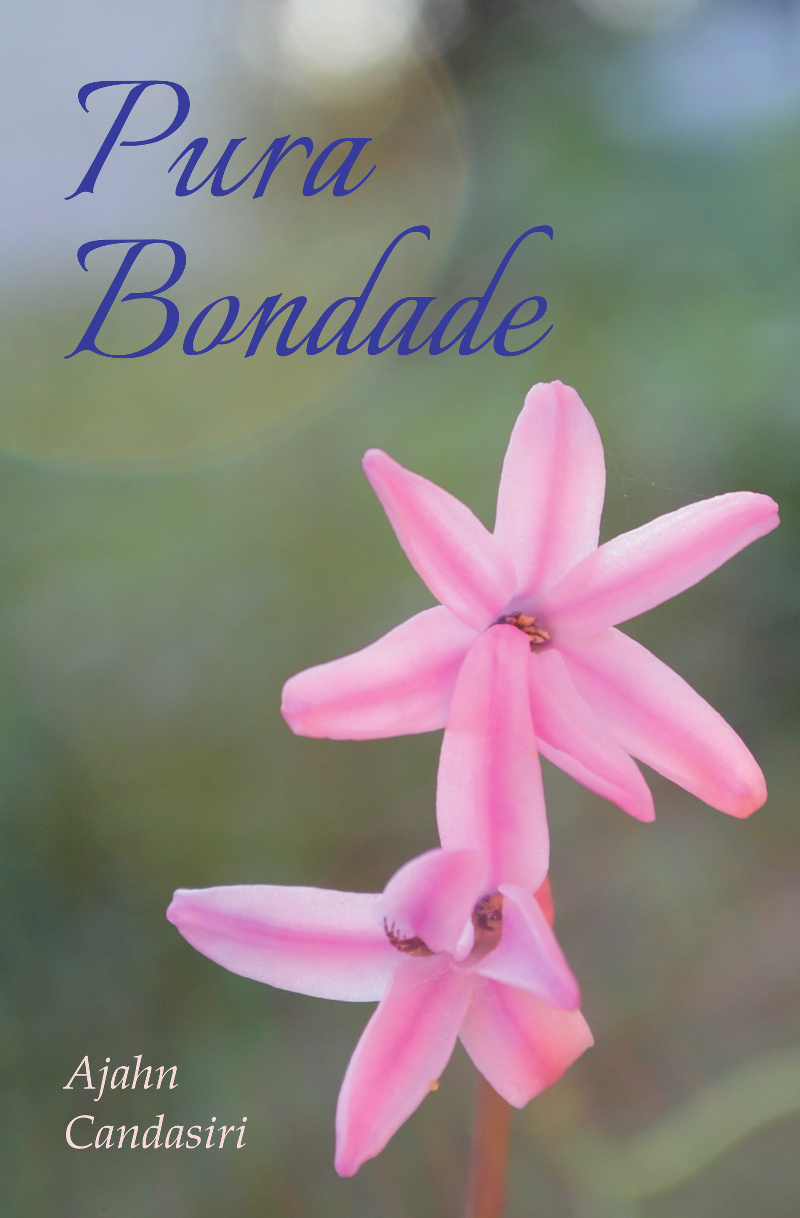
\includegraphics[height=\paperheight]{./webcover.jpg}%
}
\fi

\frontmatter

\cleartoverso
\thispagestyle{empty}

{\copyrightsize
\centering
\setlength{\parindent}{0pt}%
\setlength{\parskip}{0.8\baselineskip}%

\thetitle\\
por \theauthor

Publicações Sumedhārāma\\
\href{http://sumedharama.pt}{www.sumedharama.pt}

Para distribuição gratuita\\
\textit{Sabbadānaṃ dhammadānaṃ jinati}\\
‘A oferta de Dhamma é superior a qualquer outra oferta.’

Este livro encontra-se disponível para distribuição gratuita em\\
\href{http://fsbooks.org/}{www.fsbooks.org}

ISBN \theISBN

Copyright \copyright\ Publicações Sumedhārāma 2017

Este trabalho está licenciado com uma Licença Creative Commons\\
Atribuição-NãoComercial-SemDerivações 4.0 Internacional.

Veja página \pageref{copyright-details} para mais detalhes sobre direitos e restrições desta licença.

\theEditionInfo

Tradução: Alda Santos\\
Editor: Appamādo Bhikkhu\\
Formatação: Gambhīro Bhikkhu

Produzido com o sistema tipográfico \LaTeX.\\
Fonte utilizada: Alegreya e Crimson~Roman.

\vfill

Traduzido do original `Simple Kindness'

Publicado por Amaravati Publications\\
Amaravati Buddhist Monastery\\
Hertfordshire, Great Britain\\
publications@amaravati.org

}


\chaptertitlelefttrue

\cleartorecto
\tableofcontents*

\chaptertitleleftfalse

% Introdução
\chapter{Introdução}

Esta pequena colectânea de ensinamentos é maioritariamente composta por
palestras oferecidas num retiro de uma semana, realizado na República
Checa em 2009. A palestra final foi dada no Retiro de Final de Ano, em
2011/12, também na República Checa.

Apresentei os ensinamentos em inglês e estes foram traduzidos para
checo, para benefício da maioria dos participantes, com escassos ou
nulos conhecimentos de inglês. Isto exigiu uma precisão e economia de
palavras que descobri ser uma disciplina muito útil a partir do momento
em que me adaptei a um ritmo mais lento. Os intervalos para a tradução
também permitiram uma pausa meditativa - não constituíram, como alguns
imaginaram, momentos para pensar sobre o que dizer a seguir! A minha
ideia inicial era preparar um pequeno livro com as transcrições em
inglês e em checo, lado a lado. Posteriormente tornou-se claro que a
melhor abordagem seria preparar e editar primeiro uma versão em inglês.
É esta que o leitor tem agora nas suas mãos ( traduzida desta vez para
Português). Uma equipa de tradutores checos aguardam para posteriormente
preparar a versão checa para publicação.

Um objectivo deste livro é fornecer uma introdução para quem vai pela
primeira vez a um retiro com um professor da nossa tradição Theravada.
São apresentados os ensinamentos básicos, a par de algumas estruturas de
apoio para a prática (os Refúgios e os Preceitos), retornando a eles -
por vezes duas ou mesmo três vezes - de forma a que o leitor, ou
participante no retiro, seja constantemente lembrado dos temas
essenciais da prática. À medida que avança nestas páginas, não se
surpreenda se encontrar várias vezes tópicos como as Quatro Nobres
Verdades, impermanência, ``insatisfação'' e «não-eu», ou bondade e
curiosidade como antídotos para os cinco obstáculos.

Aqueles que já têm vários anos de prática budista contemplativa podem
igualmente encontrar alento e apoio ao regressar a estes temas básicos.
À medida que os ensinamentos são aplicados nas nossas vidas, trabalham o
coração e, gradualmente, transformam a nossa visão do mundo, pelo que,
de cada vez que os ouvimos, algo de novo é revelado.

Há mais de 2500 anos o Buddha exortou os seus discípulos «\ldots{} ide e
deambulai para o bem e a felicidade de muitos, por compaixão para com o
mundo, para o benefício, bem e felicidade dos deuses e da humanidade.» É
neste mesmo espírito que estes ensinamentos são, mais uma vez,
apresentados.

\bigskip

{\raggedleft
Irmã Candasiri\\
Rocana Vihara\\
Abril de 2012
\par}




% TODO wat.
% Faltam os ``Agradecimentos''

\cleartorecto
\thispagestyle{empty}
\vspace*{5em}
\newlength\titleLength
\newlength\xheight

{\centering

\settowidth{\titleLength}{%
  {\chapterTitleFont\Huge\itshape \thetitle}%
}

{\chapterTitleFont\Huge\itshape \thetitle}\\[0.3\baselineskip]
\setlength{\xheight}{\heightof{X}}
\raisebox{0.5\xheight}{\color[gray]{0.4}\rule{\titleLength}{0.1pt}}\\[0.3\baselineskip]
{\itshape
\thesubtitle}

\vfill

\theauthor

\vspace*{5em}

}




\clearpage
\mbox{}\thispagestyle{empty}
\clearpage

\mainmatter

% As Quatro Nobres Verdades
\chapter{As Quatro Nobres Verdades}

Há uma história, que muitos de vocês devem conhecer, que começa com o
Buddha a caminhar na floresta com alguns dos seus discípulos. A certa
altura, o Buddha baixa-se e apanha uma mão cheia de folhas do chão.
Estende as folhas aos discípulos e diz: «Digam-me se existem mais folhas
nas árvores e no chão, ou na minha mão?» Os discípulos dizem: «Existem
apenas algumas folhas na sua mão, mas existem inúmeras folhas nas
árvores e no chão da floresta.» O Buddha responde: «Sim, é verdade. As
folhas nas árvores e no chão representam todas as coisas que o Ser
Perfeito pode saber e as folhas na minha mão representam aquilo que eu
ensino: o que vocês precisam saber e contemplar, de forma a libertarem o
coração do sofrimento.»\footnote{SN 56.31, Simsapa Sutta (As Folhas de
  Simsapa).}

Alguns de vocês poderão gostar de especular sobre o início e o fim do
universo, bem como sobre todo o tipo de questões para as quais não
existe verdadeiramente uma resposta. Contudo, o Buddha encorajou-nos a
não nos preocuparmos com esses assuntos, mas antes, que tivéssemos
atenção a apenas quatro coisas, referindo-se a estas como as Quatro
Nobres Verdades. À~\mbox{primeira} chamou a Nobre Verdade do Sofrimento, a qual
se refere ao facto de nada no mundo condicionado poder proporcionar paz
ou bem-estar duradouros. Em resultado disto, a existência humana é
inerentemente insatisfatória.

Em segundo lugar, temos a Nobre Verdade da Origem do Sofrimento - esta
refere-se à existência de uma razão pela qual sofremos e ao facto de
podermos descobri-la através da nossa própria observação. Quando olhamos
cuidadosamente, podemos reparar como uma sensação de desconforto pode
criar o desejo de querer que as coisas sejam diferentes daquilo que são.
Quando nos apegamos a esse desejo, quando investimos nele, este apego
traz uma sensação de tensão, uma sensação de conflito.

A Terceira Nobre Verdade é a Verdade da Cessação do Sofrimento, do fim
da tensão ou do conflito. Isto surge quando largamos aquele desejo de as
coisas serem diferentes do que são. O desejo, em si próprio, pode
continuar, contudo nós abdicamos ou abandonamos o nosso empenho nele.
Fazemos as pazes com a realidade tal como ela é.

A Quarta Nobre Verdade é a Nobre Verdade do Caminho que Conduz ao Fim do
Sofrimento: consiste nas orientações que o Buddha nos deixou sobre como
viver a nossa vida de forma a sofrermos cada vez menos.

No decurso deste retiro iremos contemplar estas verdades apresentadas
pelo Buddha. Se estamos a sentir sofrimento, podemos dar por nós a
pensar que temos de fazer alguma coisa, que temos de escapar ao
sofrimento, mas o Buddha disse: «Não, o sofrimento deve ser
compreendido.» Não conseguimos compreender o sofrimento nas nossas vidas
se estamos constantemente a tentar fugir dele ou a distrairmo-nos. Por
isso aquilo que proponho é que, ao longo destes dias, se interessem,
sejam curiosos relativamente à vossa vida e experiência - incluindo
mesmo as tensões, as pressões e lutas aparentemente triviais ou as
formas subtis de aversão ou negatividade. Interessem-se verdadeiramente
pela forma mais insignificante de ansiedade ou de medo, como um
cientista a examinar algo ao microscópio.

Há pouco, quando fui dar uma volta a pé, reflecti em como fazer um
retiro é um pouco como estar de férias e fazer amizades. Isto pode
parecer um pouco surpreendente aos que estão habituados ao tipo de
retiros nos quais são encorajados a trabalhar arduamente, nos quais é
enfatizado o esforço despendido para progredir na prática da meditação.
Também podem interrogar-se sobre o que quero dizer com «fazer amizades»
quando praticamos o Silêncio Nobre: não falar uns com os outros a não
ser que seja mesmo necessário. Com efeito, o que eu gostava de encorajar
o mais possível é que alcancem uma sensação agradável, de tranquilidade
e descontracção. Não me refiro ao tipo de relaxamento que leva a que
simplesmente adormeçam, apesar de alguns de vocês poderem sentir muita
sonolência nos primeiros dias. Este tipo de tranquilidade e
descontracção a que me refiro é um estado de vigília, uma inteligência,
e o tipo de amizade que sugiro é que tentem ser mais amigáveis com vós
próprios.

Uma das coisas mais tristes e difíceis para as pessoas na nossa cultura
ocidental parece ser a falta de capacidade de fazerem amizade consigo
próprias, para se aceitarem tal como são. Podemos ser bondosos para com
as outras pessoas, perdoá-las e aceitá-las, mas quando olhamos para as
nossas mentes e para a forma como nos relacionamos connosco próprios,
vemos que, frequentemente, podemos ser muito cruéis, muito exigentes e
severos nos juízos sobre nós mesmos. Por isso encorajo-vos a
conhecerem-se melhor nestes próximos dias, de uma forma mais gentil.
Reparem naquilo que não gostam e que não aprovam em vós próprios, e
vejam apenas se se podem perdoar e aceitar as coisas tal como são. Desta
forma pode dar-se uma verdadeira transformação. Do mesmo modo,
apercebo-me que quanto mais faço amizade comigo própria, mais apta estou
a fazer amizade com outras pessoas.

Se insistimos em reprimir o que não nos agrada, os nossos pensamentos e
as nossas disposições desagradáveis, não nos estamos a aceitar realmente
e provavelmente acabaremos por adoecer. Parece que grande parte das
doenças dos tempos atuais resulta de não cuidarmos adequadamente da
nossa vida emocional.

Por isso, podemos ver este tempo de retiro como uma oportunidade de
fazer algum trabalho preventivo importante. Se criarmos uma atmosfera
interna de confiança e de bondade, os nossos maus hábitos de pensamento
podem revelar-se. Então, tendo visto e admitido estes hábitos, podemos
abrir mão deles, de forma que as nossas vidas deixem de ser limitadas
pelos seus efeitos negativos.



% Os Três Refúgios e Os Cinco Preceitos
\chapter{Os Três Refúgios e Os Cinco Preceitos}

As palavras \emph{Buddha}, \emph{Dhamma} e \emph{Sangha} são
frequentemente usadas na nossa prática. A palavra \emph{Buddha}
refere-se ao professor histórico, significando igualmente a nossa
própria capacidade para despertar, a capacidade de ver as coisas
claramente. O \emph{Dhamma} é o ensinamento dado pelo Buddha, que aponta
para a verdade que cada um de nós pode apreciar ou saber por si próprio,
quando nos encontramos completamente presentes ou na realidade tal como
é. O \emph{Sangha} é a comunidade dos discípulos do Buddha - gerações
incontáveis de homens e mulheres, desde o tempo do Buddha, que ouviram
os ensinamentos e que, através da sua aplicação nas suas vidas, têm sido
capazes de compreender a verdade por eles próprios e experimentar paz
nos seus corações. A palavra \emph{Sangha} pode igualmente referir-se à
comunidade de pessoas que se apoiam mutuamente na sua prática, tal como
nós nos apoiamos mutuamente durante este retiro.

Chamamos ao Buddha, ao Dhamma e ao Sangha os \emph{Três Refúgios}. Estes
podem igualmente ser chamados as Três Jóias ou a Gema Tripla. Uma jóia é
algo requintado que não pode ser danificado, o que constitui uma
comparação útil, uma vez que podemos confiar sempre nestes três refúgios
- eles estão sempre presentes, independentemente de onde quer que vamos
e do que façamos. Por isso, encorajo-vos a reflectirem sobre estes
tesouros sem preço, estes refúgios - é desta forma que eles poderão vir
a ter um significado e um valor reais nas vossas próprias vidas.

O apoio tradicional para aqueles que escolhem seguir os ensinamentos do
Buddha são estes três refúgios, juntamente com os Cinco ou os Oito
Preceitos. Os Cinco Preceitos são as directrizes éticas que o Buddha
recomendou e encorajou para os leigos, nas suas vidas do dia-a-dia. Os
Oito Preceitos são para os noviços ou para os visitantes de um mosteiro
- são, de igual forma, geralmente utilizados como apoio num período de
retiro. O Primeiro Preceito envolve a abstenção de matar - não tirar a
vida a nenhum ser, mesmo a criaturas minúsculas que nos desagradam.
Podemos usar este preceito como uma directriz para nós próprios.
Contudo, se acidentalmente fizermos mal a um insecto, apesar de ser
lamentável, não constitui uma quebra deste Preceito. O Preceito apenas
quer dizer que nos devemos abster de, intencionalmente, causar qualquer
mal ou matar qualquer ser vivo. Em segundo lugar abstermo-nos de retirar
seja o que for que não nos tenha sido dado ou disponibilizado para
utilizarmos. Nós não roubamos. Este Preceito é muito útil porque
significa que podemos viver juntos e confiar uns nos outros, o que é
algo bonito.

O Terceiro Preceito é abstermo-nos de qualquer actividade sexual
intencional. Quando inserido nos Cinco Preceitos, traduz-se na abstenção
de qualquer conduta sexual danosa. Devemos compreender que este Preceito
não constitui uma proibição relativa ao desejo sexual - toda a gente
sente, naturalmente, desejo sexual. Aquilo que nos é pedido é para nos
abstermos de agir de acordo com esse desejo ou, no caso dos Cinco
Preceitos, de procurar qualquer forma de gratificação sexual com alguém
com quem não tenhamos uma relação que envolva um compromisso.

O Quarto Preceito trata de nos abstermos do discurso incorrecto. No
contexto dos Cinco Preceitos isto pode ser interpretado como o cultivo
do discurso cuidado e a abstenção dos quatro tipos de discurso danoso: a
mentira, a intriga, a palavra rude ou danosa e o tagarelar frívolo.
Quando fazemos um retiro, em geral é-nos pedido que observemos o Nobre
Silêncio, uma vez que, quando mantemos o silêncio externamente, temos
uma boa oportunidade para escutar o tagarelar interno da mente. Espero
que tenham igualmente oportunidade de observar como esse tagarelar
começa a acalmar, nem que seja apenas um pouco. Alguns de vocês vão
sentir uma grande paz. Para outros podem ser apenas alguns momentos aqui
e ali. Quer se trate de uma grande paz ou apenas de uma pequena paz, não
tem importância. O que importa é estar presente e reparar no que está a
acontecer. Não existe um prémio para a mente que conseguir estar mais em
paz!

O Quinto Preceito envolve a abstenção de tomar qualquer tipo de
intoxicantes - álcool ou drogas recreativas. Se necessitarem de tomar
algum medicamento que vos tenha sido prescrito, óptimo - e tenho o
prazer de vos dizer que a cafeína também é permitida.

O Sexto Preceito envolve a abstenção de comer depois do \mbox{meio-dia}, ou em
alturas inapropriadas. A ideia é não utilizar a comida como uma forma de
distracção. Recordo-me que, quando era leiga, sempre que me sentia um
pouco entediada ou infeliz, lançava automaticamente a mão a qualquer
coisa comestível. Contudo, durante este retiro peço-vos para não fazerem
e, em vez disso, observarem o sentimento, seja ele qual for, de
aborrecimento ou infelicidade que poderão estar a experienciar, bem como
para repararem como é que esse sentimento se altera. Desta forma poderão
ter uma compreensão profunda da impermanência - podem observar,
realmente, por vocês próprios, como as coisas se modificam.

O Sétimo Preceito consiste na abstenção relativamente a entretenimentos,
embelezamento e adornos. Não usamos grinaldas no nosso cabelo ou outro
tipo de jóias (alianças são permitidas) e não participamos em desportos
ou jogos, nem ouvimos música ou praticamos qualquer das actividades que,
em geral, são consideradas divertimento. Em vez disso, temos uma
oportunidade de experienciar um tipo de prazer muito mais subtil - e
divertido - através da nossa meditação.

O Oitavo Preceito consiste na abstenção de nos deitarmos numa cama
elevada ou luxuosa, o que pode soar um pouco estranho. No entanto,
trata-se de um estímulo no sentido do cultivo de uma atitude de vigília,
em vez da utilização do sono como uma fuga ou da procura do prazer
através da posse de mobiliário luxuoso. Isto não significa que não
possamos descansar ou que não devamos dormir; apenas que descansamos na
medida em que isso é necessário. Podemos aprender muito estando
acordados e atentos ao que ocorre nas nossas mentes e nos nossos corpos.

É importante ver estes Preceitos como apoios amigáveis, ao invés de
agentes da polícia secreta que vão estar a vigiar-nos e a \mbox{punir-nos} se
cometermos algum erro. Eles estão disponíveis para serem usados por nós,
nas nossas vidas, se assim escolhermos. Os Cinco Preceitos são um
lembrete para nos mantermos no âmbito de fronteiras éticas, de forma
que, tanto quanto possível, evitemos comportamentos que sejam danosos
para nós ou para os outros - comportamentos que nos metam em apuros. No
retiro, os restantes Preceitos de Renúncia contribuem para a
simplificação. Fazemos uma escolha consciente em não participar em
determinadas actividades. Através desta escolha criamos o espaço dentro
de nós. Podemos então observar directamente as nossas formas habituais
de perceber e de responder às experiências. Desta maneira podemos ver o
que é necessário para libertar o coração do sofrimento.



% Curiosidade e Compreensão
\chapter{Curiosidade e Compreensão}

Ao chegarmos ao final do primeiro dia de prática, é interessante reparar
nos efeitos deste tipo de esforço. Cada um pode reparar quão diferente
se sente em relação a como se sentia ontem por esta hora, quando aqui
chegaram. Vejo que estão mais ambientados e, talvez, um pouco cansados.
Isto é normal, uma vez que também vejo que todos se têm aplicado muito
na prática da meditação. Por vezes a meditação requer mesmo que nos
apliquemos bastante. Esta noite gostava de vos falar sobre diferentes
tipos de compreensão. A palavra ``compreensão'' pode ser usada para
\emph{qualquer} tipo de constatação - um daqueles momentos de «ahhhh»
quando, de repente, vemos as coisas de forma diferente, quando temos uma
compreensão diferente. A compreensão pode ser acerca de coisas bastante
vulgares. Como exemplo, gostava de vos falar de uma compreensão que me
ocorreu, recentemente, acerca de algo pequeno e prático. Relaciona-se
com a casa, ou \emph{kuti}, onde vivo. Trata-se de um \emph{kuti} muito
simpático, que foi construído há cerca de catorze anos por uma das
monjas; está ainda em muito boas condições. Contudo, há alguns anos
comecei a notar que existiam algumas criaturas a viver nas paredes e no
tecto. Não tinha a certeza do que eram, mas desde que tivemos um
problema com ratazanas no mosteiro, aqueles que organizam o trabalho
partiram do princípio que se tratava de uma ratazana e resolveram pôr
rede de arame à volta da base do meu \emph{kuti}, em todos os sítios por
onde uma ratazana pudesse entrar. Fizeram um excelente trabalho\ldots{}
mas, claramente, as criaturas ainda viviam lá felizes e contentes.

Foi para mim um quebra-cabeças tentar descobrir como é que entravam e
saíam.Nos último meses tornaram-se muito mais activas, de uma forma
bastante desagradável. Ao princípio costumava achar que elas eram
bastante amorosas, mas agora acho-as verdadeiramente intrusivas, por
isso estava decidida a descobrir como é que elas entravam e saíam, de
forma a poder fazer qualquer coisa para as impedir. Pensei que talvez
estivessem a escavar túneis por baixo do \emph{kuti}, de forma que
sempre que encontrava um buraco que parecesse uma possibilidade nesse
sentido colocava uma pedra sobre ele. Mas elas continuavam lá. Então
comecei a ouvir atentamente. Parecia que estavam a saltar para o
telhado, vindas das árvores mais próximas. Pedi a alguém que cortasse os
ramos das árvores, de forma que não pudessem ter esse acesso ao telhado.
Mas isso também não resultou, elas continuavam lá. Então ouvi dizer que
existem ratazanas que conseguem trepar pelas paredes dos edifícios.
Pensei que estas deviam ser dessa espécie, por isso despendi muito tempo
a ver se existiam quaisquer buracos na parte de baixo do telhado. Mas
trata-se de um \emph{kuti} muito bem construído, e não consegui
encontrar quaisquer buracos. Então comecei a olhar para as telhas para
ver se as ratazanas poderiam entrar por baixo delas, mas também não
consegui ver aí quaisquer buracos.

Eventualmente, em desespero, subi por um escadote de forma a olhar
devidamente para o telhado. Então surgiu o momento da compreensão:
\emph{Ahhhh!} Vi três buracos grandes na base da chaminé. Assim, quando
achei que as ratazanas tinham saído, fechámos esses buracos. Mas a
história não acaba aqui, porque nessa noite houve muita agitação e o som
de qualquer coisa a roer a parede ou o telhado. Bem, isso confirmava que
era pelos buracos que elas entravam \emph{e} saiam. De forma que ainda
não tínhamos conseguido resolver o que fazer. Destapámos os buracos e eu
estou apenas à espera que saiam - e a entoar um cântico intitulado o
cântico de proteção das cobras:

\begin{quote}
  \itshape
  Gosto dos animais sem pés\\
  Gosto dos animais com dois pés\\
  Gosto dos animais com quatro pés\\
  Gosto dos animais com muitos pés\\
  Mas por favor vão-se embora.
\end{quote}

Espero que isto vos dê uma ideia de um momento de compreensão, de quando
estamos perplexos relativamente a algo, investigamos verdadeiramente e
\emph{depois} vemos. Com a nossa prática \mbox{aplica-se} o mesmo princípio. Os
ensinamentos do Buddha existem para nos encorajar e mostrar para onde
dirigir as nossas vidas. Podemos estudar muitas escrituras de forma a
conseguir uma compreensão intelectual, mas sinto que todos aqui estão
interessados em algo mais nutritivo para o coração, de outra forma
estariam todos na universidade a estudar Budismo!

Quando ouvi pela primeira vez ensinamentos budistas, na realidade não me
apercebi que se tratava de Budismo; pareceram-me apenas senso comum e
fiquei muito entusiasmada relativamente à possibilidade de
\emph{descobrir} realmente a verdade por mim própria. Assim, ao virmos
fazer este retiro, temos uma oportunidade de contemplar os ensinamentos
em relação à nossa própria experiência. Aqui, a teoria e a prática
encontram-se e, quando nos aplicamos, a compreensão pode surgir.

Uma coisa que tenho notado relativamente às compreensões é que estas
muitas vezes surgem de forma bastante inesperada. Podemos sentar-nos ou
fazer meditação a andar durante horas e nada acontece. Mas depois,
quando estamos a fazer qualquer coisa muito normal, como lavar os
dentes, vestir-nos ou sair para andar um pouco - de repente, há
compreensão. Vemos o que um determinado ensinamento quer dizer -
torna-se real para nós.

O Ajahn Chah contou uma história sobre uma compreensão que certa vez
teve: ele queria fazer um hábito para si próprio; ora, os nossos hábitos
têm um modelo especial - são cozidos de uma forma particular, bastante
complicada. Então Ajahn Chah passou o dia inteiro a pensar nisso e,
finalmente, conseguiu perceber através do seu raciocínio, como fazer o
hábito. Com esta experiência Ajahn Chah constatou que, quando estamos
realmente interessados em qualquer coisa, de forma natural aplicamos o
nosso raciocínio e, a seu tempo, surge a compreensão. É por isso que dou
sempre ênfase e encorajo uma atitude de curiosidade - sermos curiosos
relativamente à nossa experiência. Se realmente nos interessarmos e
aplicarmos o nosso esforço a investigar a vida, começamos a compreender.

Podemos ter compreensões relativamente a muitas coisas, algumas das
quais são úteis do ponto de vista da libertação, enquanto outras não o
são de todo. Penso que todos nós, aqui presentes, estamos interessados
no tipo de compreensões que nos trarão liberdade ao coração, que nos
libertem o coração. Queremos compreender a razão pela qual sofremos.
Porque é que existe sofrimento? Queremos compreender como libertar o
coração do sofrimento. Bem, viemos ter ao lugar certo, porque o Buddha
disse: «Ensino sobre o sofrimento e sobre o fim do sofrimento.»

Falei ontem das Quatro Nobres Verdades. Para cada uma das verdades o
Buddha apontou três aspectos. O primeiro aspecto da Primeira Nobre
Verdade é que existe sofrimento. O segundo aspecto é que o sofrimento
precisa de ser compreendido, depois vem a realização libertadora de que
o sofrimento \emph{foi} compreendido. Se queremos compreender algo, é
necessário que estejamos dispostos a examiná-lo. Contudo, esta não é a
resposta comum ao sofrimento. Em geral, quando existe sofrimento,
queremos ver-nos livres dele tão depressa quanto possível, não queremos
examiná-lo. Mas se seguirmos a prática como o Buddha ensinou, torna-se
claro para nós que, se queremos libertar o coração do sofrimento será
necessário examiná-lo - precisamos de o compreender. Podemos passar toda
a nossa vida a tentar distrairmo-nos do sofrimento, mas isso não faz com
que estejamos mais perto da libertação do coração.

Fiz o meu primeiro retiro com o Ajahn Sumedho há cerca de trinta anos,
como leiga. Na minha entrevista ele perguntou como é que eu estava.
Disse-lhe que gostava muito do retiro, estava a gostar muito da
estrutura do retiro\ldots{} e então desatei a chorar e dei por mim a
dizer: «Mas tenho este orgulho. Não consigo \mbox{ver-me} livre dos pensamentos
de orgulho!» Eu pensava realmente que não devia ter estes pensamentos e
queria desesperadamente ver-me livre deles. Ajahn Sumedho e o monge que
o acompanhava ficaram muito silenciosos. Passados uns momentos Ajahn
Sumedho disse-me: «Não é o \emph{orgulho} que é o problema. É \emph{não
o querer}.» Este foi um momento importante para mim. Vi claramente a
distinção entre aquilo que estava a acontecer na minha mente e a minha
reacção a isso. Pude ver que existia uma distinção clara entre a
condição desagradável e o sofrimento. Comecei a ver que, mesmo com
situações desagradáveis da mente ou do corpo, podemos, na realidade,
estar bastante serenos. Tornou-se claro que o sofrimento não era causado
pela própria condição mas pela luta no sentido de evitar essa condição.

Querer que as coisas sejam distintas daquilo que são, envolvermo-\linebreak -nos no
desejo de que as coisas sejam diferentes, leva-nos ao stress, à luta, ao
sofrimento. Mas se pudermos reconhecer a condição desagradável e
simplesmente admitirmos que existe um desejo natural de querer evitá-la,
podemos alcançar uma condição de paz real. Isto também funciona com
condições agradáveis: temos a tendência de nos agarrarmos a elas, não
queremos que elas se alterem mas, é claro que também elas mudam. Desta
forma, também podemos sofrer com condições agradáveis, se não
compreendermos e aceitarmos realmente o facto da mudança.

Durante este retiro temos a oportunidade de investigar a nossa
experiência, para sermos verdadeiramente curiosos e interessarmo-nos
pelas nossas respostas às diferentes situações que surgem. Por exemplo,
alguns de vocês não estão muito bem, estão constipados ou têm a febre
dos fenos, e portanto podem notar o tipo de negatividade e de aversão
que surge em resposta às sensações físicas desagradáveis - e,
evidentemente, que o mesmo se aplica a condições mentais desagradáveis.

Um outro aspecto importante da compreensão relaciona-se com
\emph{annica}, impermanência, mudança. Uma vez estava a fazer uma
caminhada com um grupo de leigos. Estávamos a caminhar há cerca de uma
semana numa zona de campo muito bonita, no norte de Inglaterra. Um dia,
estava junto a uma cascata a observar o movimento e os padrões da água
que caía. Ocorreu-me um poema, e constatei que na realidade este
reflectia a vida:

\begin{quote}
  \emph{A cair}\\
  \emph{A cair}\\
  \emph{Posso apanhar?}\\
  \emph{Posso apanhar?}\\
  \emph{Não\ldots{}}\\
  Não podemos!
\end{quote}

Nas nossas vidas por vezes experienciamos coisas lindíssimas. Temos
também relacionamentos especiais, nos quais sentimos uma afinidade
maravilhosa e um grande à-vontade com determinadas pessoas. Pode
acontecer o desejo de nos agarrarmos a essas experiências. Mas
precisamos compreender que a vida envolve uma espécie de
implacabilidade. É \emph{annica} - simplesmente continua a fluir, quer
queiramos ou não.

O \emph{Dhammacakkappavattana Sutta} é o primeiro sermão do Buddha
depois do seu despertar. Nele o Buddha fala acerca das Quatro Nobres
Verdades e dos seus três aspectos - este \emph{sutta} tem uma quantidade
imensa de ensinamentos. Diz-se que depois do Buddha ter apresentado este
ensinamento, o Venerável Kondañña, um dos cinco ascetas que se
encontravam a ouvir, \emph{compreendeu}. O sutta prossegue dizendo que
ele compreendeu que: «Tudo o que tem a natureza de surgir tem a natureza
de cessar.» Gosto muito desta simplicidade. Somos também informados que,
quando o Venerável Kondañña compreendeu isto, todos os \emph{devas},
todos os anjos de todos os reinos celestes se regozijaram. Os
\emph{devas} terrenos gritaram para o nível seguinte: «O Venerável
Kondañña compreendeu! Ele percebeu!» e o regozijo ascendeu através de
todos os diferentes níveis dos reinos dos \emph{devas} e o mundo de dez
mil sistemas agitou-se, abanou e estremeceu. Houve uma enorme tempestade
e um esplendor sem limites invadiu todo o universo - tudo devido à
compreensão do Venerável Kondañña de que tudo o que tem a natureza de
surgir tem a natureza de cessar. Para alguns de vocês esta compreensão
pode parecer pouco importante, mas foi obviamente muitíssimo
significativa. É algo que podemos contemplar ao longo destes dias, de
forma a que compreendamos que tudo - estes corpos, estas mentes, os
estados de espírito, os estados do corpo - está em constante mudança.

Uma das coisas que aprecio quando regresso a este centro de retiros é
ter a oportunidade de ver as mudanças: as árvores que se plantaram a si
próprias no rio, a crescer, o edifício a degradar-se, as modificações
nas pessoas que encontro ano após ano e ver a minha própria cara no
espelho, ver como se altera. Para pessoas que não contemplam o
\emph{Dhamma}, ver a cara a mudar com a idade pode ser um mau prenúncio.
Mas eu gosto bastante.

Para concluir, as compreensões libertadoras relacionadas com as Quatro
Nobres Verdades são compreensões relativas às três características de
todas as condições: tudo é impermanente (\emph{anicca}), tudo é
inerentemente insatisfatório (\emph{dukkha}) e não existe qualquer
pessoalidade permanente seja no que for (\emph{anatta}). Existe uma
frase que aprecio muito nos cânticos da manhã: «Para a total compreensão
disto, durante a sua vida, o Abençoado instruiu frequentemente os seus
discípulos neste sentido.» Entoamos este cântico praticamente todos os
dias no mosteiro. Acho este cântico diário muito útil pois este
ensinamento pode levar algum tempo até ser realmente compreendido.

A minha expectativa para estes dias de retiro é que, na meditação, todos
experienciem alguma calma, alguns estados de espírito agradáveis, e
espero igualmente que todos tenham uma pequena compreensão relativamente
à natureza do sofrimento e à possibilidade de o coração se libertar
dele.



% Os Cinco Obstáculos
\chapter{Os Cinco Obstáculos}

Estamos a praticar em conjunto há alguns dias. Até agora, tem sido dada
maior enfâse à meditação focada na serenidade e também falei um pouco
sobre as compreensões. Muitos de nós, principalmente os que já praticam
há algum tempo, têm já uma noção clara daquilo que é necessário. Mas,
apesar da prática ser simples, nem sempre é fácil. Isto acontece devido
aos hábitos da ignorância e da ilusão (que nos têm condicionado desde
que nascemos) serem muito fortes. Queremos muitas coisas e não queremos
muitas outras. Em geral temos alguma confusão relativamente ao que é bom
para nós e, por isso, fico sempre grata ao Buddha por ter formulado de
modo tão claro os ensinamentos e a forma de praticar.

Muitos de vocês têm noção de que no Budismo existem muitas listas. Isto
aconteceu porque no tempo do Buddha os ensinamentos não eram escritos,
não havia qualquer registo e as pessoas não tomavam notas como hoje em
dia fazemos. Elas \mbox{reuniam-se} em redor do Buddha, escutavam os seus
ensinamentos e memorizavam-nos. Aparentemente as pessoas desses tempos
tinham memórias prodigiosas, podiam lembrar-se de um número formidável
de coisas. Penso que os registos e os computadores, e esse tipo de
coisas que temos hoje em dia, nos tornaram um pouco preguiçosos -- os
nossos cérebros não têm a mesma capacidade, não temos tanta memória.
Mais facilmente confiamos na memória do nosso computador! Mas, naqueles
tempos, os discípulos do Buddha lembravam-se dos ensinamentos e, quando
estavam em viagem ou longe do Buddha, repetiam-nos para as pessoas que
se reuniam para ouvi-los. Os ensinamentos foram transmitidos desta forma
durante várias centenas de anos, antes de terem sido compilados e
escritos. Isto parece completamente espantoso quando vemos as
colectâneas das escrituras do Buddha pois contêm milhares de páginas e
uma quantidade vastíssima de informação.

Uma das listas, que considero muito útil na minha prática, é a que se
refere aos Cinco Obstáculos. Esta lista explica, de forma muito clara, a
razão pela qual, por vezes, apesar de sabermos o que \emph{devíamos} de
fazer, não o conseguimos fazer. Estes obstáculos são impedimentos.
Dificultam-nos a meditação. Mas quando temos consciência dos obstáculos,
podemos ver o caminho através deles e então, ao invés de obstáculos,
eles podem levar-nos a um estado de maior discernimento e de compreensão
mais profunda. Assim, na realidade, eles podem por vezes ser muito
úteis, uma vez que tenhamos aprendido a reconhecê-los. Primeiro vou
\mbox{enumerá-los} e depois falarei um pouco sobre cada um deles. Penso que
reconhecerão alguns, senão todos, na vossa própria prática.

\begin{quote}
  O primeiro obstáculo na lista é o desejo sensorial, a ânsia sensorial.

  O segundo obstáculo é a má vontade, a negatividade, a aversão.

  O terceiro obstáculo é a sonolência e a lentidão (preguiça e torpor).

  O quarto obstáculo é a inquietação e a agitação da mente -- uddhacca-kukkucca em Pali.

  O quinto obstáculo é a dúvida.
\end{quote}

Tal como referi, quando os reconhecemos claramente, deixam de ser
obstáculos, uma vez que nessa altura existem maneiras muito claras de
trabalhar cada um deles. Só são obstáculos quando ainda não os tornámos
conscientes, quando ainda não estamos realmente conscientes do que está
a acontecer. Metemo-nos em sarilhos quando os seguimos ou somos levados
a reagir a eles. É aí que eles nos prendem e evitam que vejamos as
coisas claramente.

Uma das coisas mais difíceis no que diz respeito aos obstáculos, é que
temos tendência a complicá-los, por lhes termos aversão.

Podemos transtornar-nos por sermos gananciosos. Sentimos que não
deveríamos ser gananciosos e, por isso, detestamo-nos. Detestamos ser
irritáveis e rabugentos e negativos. Podemos sentir-nos completamente
desesperados com a nossa molenguice e sonolência, podemos sentir-nos
completamente frustrados e perturbados com a nossa mente inquieta e
agitada e podemos debater-nos seriamente com a dúvida, não a querendo,
não gostando dela. Assim, complicamos ainda mais estas condições com a
nossa aversão e resposta negativa a elas. Mas quando simplesmente
reconhecemos a ganância, a negatividade, a preguiça, a inquietação e a
dúvida -- quando podemos reconhecê-las por aquilo que são, em vez de as
encararmos como um problema, algo que não deveríamos ter ou uma qualquer
falha básica no nosso carácter -- tornam-se um quebra-cabeças ou um
desafio interessante, uma parte do jogo da vida. Podem até tornar-se
divertidas.

Evidentemente, nem sempre é fácil vê-las sob este prisma e por vezes
necessitamos de um amigo próximo que nos ajude a ver as coisas de forma
diferente. Essa é uma das maiores bênçãos de viver num mosteiro. A maior
parte dos monges e das monjas, particularmente os que já lá se encontram
há muito tempo, já perderam um pouco o idealismo relativamente a eles
próprios ou a qualquer pessoa. Já não têm expectativas no sentido de
serem sempre perfeitos. São capazes de reconhecer e aceitar os
obstáculos e compreendem que estes são uma parte natural da condição
humana. Não algo a ser detestado ou temido, mas sim algo a ser
compreendido e trabalhado de forma positiva.

Em Chithurst, nos primeiros tempos, todos trabalhávamos arduamente. A
casa encontrava-se praticamente em ruínas e tivemos de a reconstruir. O
jardim estava uma selva. Éramos quatro monjas noviças e costumávamos
cozinhar para todos. Por vezes não havia muito para cozinhar: teríamos
feijões e arroz e urtigas e, talvez, uma cebola. Era muito divertido,
mas a nossa meditação não era grande coisa (!) Estaríamos todas
sentadas a cabecear e sonolentas! Lembro-me do Ajahn Sucitto, um dos
monges seniores, elogiar-nos e encorajar-nos. Ele dizia que devíamos
comemorar o facto de, pelo menos, conseguirmos manter-nos sentadas sem
bater com as cabeças no chão. Quando vivemos numa comunidade de
praticantes, é possível rir (acerca) destas coisas, não as levando
demasiado a sério. Mas quando não temos este tipo de apoio, podemos
sentir-nos muito desesperados quando experienciamos estados de ganância,
estados de negatividade ou estados de embotamento. Só o simples facto de
conseguirmos notar o que se está a passar, pode requerer, uma tremenda
quantidade de compaixão e de ternura para connosco.

Creio que a razão pela qual muitos de nós procura a meditação prende-se
com o facto de querermos tornar-nos pessoas melhores. Mas, claro que,
como provavelmente se aperceberam, assim que começamos a meditar tomamos
consciência de todas as coisas menos boas acerca de nós próprios. Quando
era leiga costumava pensar que era uma pessoa bastante pacífica. As
pessoas diziam: «Ela é tão calma, tão tranquila.» Mas quando me tornei
monja descobri uma raiva imensa; por vezes apetecia-me bater nas pessoas
ou desejava que não existissem! Por isso poderiam pensar que, talvez, eu
não devesse ter começado a meditar, mas discordo com veemência. Penso
que é muito bom meditar. Podemos encarar a meditação como um processo de
descontracção interna. Somos educados para sermos bem comportados e
bons, de modo que aprendemos a reprimir ou ignorar as nossas qualidades
desagradáveis. Depois, à medida que começamos a meditar, descontraímos
e, assim, estas coisas começam a vir à superfície. No Budismo falamos
sobre purificar o coração e fazemos isto ao permitir que todas estas
coisas, que não parecem assim tão puras nem encantadoras, venham ao de
cima. Então podemos largá-las. Por vezes, descobrimos que posteriormente
temos muito mais energia, pois já não estamos a despender muito esforço
a tentar manter tudo sob controlo.

Os Cinco Preceitos são uma protecção. Quando os adoptamos abstemo-nos de
matar, de roubar, de ter uma conduta sexual danosa, de ter um discurso
incorrecto e de consumir substâncias intoxicantes. São como cinco bons
amigos que nos recordam o cuidado a ter com as energias do desejo, da
luxúria, da negatividade, do ódio e da aversão. Assim, quando estas
energias surgem, podemos simplesmente reconhecê-las e tratá-las com
cuidado e respeito, uma vez que podem causar bastantes danos. E, à
medida que as vamos compreendendo e percebendo como lidar com elas,
deixamos de ter medo delas. Quando, através da nossa investigação, se
torna claro que são \emph{anicca}, \emph{dukkha}, \emph{anatta} - mudam,
são insatisfatórias e não são quem somos - deixamos de precisar de nos
identificar com elas e, então, de certa forma, libertamo-nos delas.
Mesmo que elas possam lá estar, já não estamos presos ao desejo de as
seguir, de agir de acordo com elas. Temos escolha.

Nas escrituras, o Buddha dá uma série de ensinamentos sobre os
obstáculos e as diferentes formas de trabalhar com eles, utilizando
comparações muito úteis, para nos dar uma ideia do que são e de como nos
afectam.

A má vontade ou negatividade, disse o Buddha, é como uma doença. Durante
os retiros é muito importante estar atento às diferentes formas de
negatividade, particularmente a negatividade dirigida a nós próprios.
Podemos ser muito duros connosco próprios, muito intolerantes. Parecemos
ter muita destreza para ver os nossos defeitos, para reconhecer as
coisas que fizemos mal mas, por vezes, temos uma verdadeira dificuldade
em celebrar as coisas que fazemos bem. Isto é algo ao qual temos de
estar atentos e no qual temos de reparar.

Estes obstáculos podem ser muito grandes, muito radicais, mas podem
igualmente ser muito subtis. Por vezes, é mais difícil lidar com as
formas mais subtis de negatividade. A raiva é muito óbvia, mas a pequena
irritação ou a rabugice podem, à partida, ser mais difíceis de
reconhecer. Uma das coisas que tenho reparado na minha própria prática
no que respeita à rabugice ou à irritabilidade é que, com frequência,
acho que não as devia sentir. Contudo, aprendi ao longo dos anos a
simplesmente reconhecer quando me sinto rabugenta. Por vezes, digo mesmo
às pessoas: «Não falem comigo hoje, estou a sentir-me rabugenta.» E, por
vezes, se alguém que conheço muito bem fala comigo de coisas que me
perturbam, então digo-lhe: «Não estou com disposição para falar disso
agora.»

Assim, é realmente útil reconhecer quando existe negatividade ou aversão
na mente pois de outra forma esta pode facilmente intensificar-se e
afectar os outros. Lembro-me uma vez, de estar a conversar com alguém
sobre um assunto no qual não estava particularmente interessada, mas fiz
um comentário qualquer e a pessoa discordou de mim. Então,
automaticamente, eu discordei dela e depois ela discordou de mim! E dei
por mim a ficar cada vez mais zangada e desagradada. Eventualmente vi o
que estava a fazer e descontraí-me. Reconheci aquele sentimento de ter
de vencer uma discussão com alguém e pensei: «Na realidade não tenho de
fazer isto.»

Fiquei muito impressionada com um grupo de pessoas que trabalham na
Palestina, para ultrapassar os conflitos entre os palestinianos e os
israelitas. O seu lema é «A Paz é o mais importante.» Apesar disto me
fazer todo o sentido, podia ver que a prática destas pessoas era muito
exigente. Estabelecer a paz significa abdicar de ou renunciar à posição
de ter razão. É um verdadeiro sacrifício do ego, do sentido de si
próprio. E, devido à forma como fomos condicionados, o sentido de si
próprio é \emph{muito} importante para nós. Apesar de ser apenas uma
ilusão, fazemos tudo o que está ao nosso alcance para nos agarrarmos a
ele, até nos apercebermos de todos os problemas que causa, tanto a nós
como aos outros.

Assim, a negatividade ou a má vontade é como uma doença.

O Buddha disse que o desejo sensual é como estar em dívida, sentir que
se tivéssemos aquilo que queremos seríamos completos e felizes. Mas
\emph{nunca} nos sentimos completos, queremos sempre cada vez mais e
melhor - quer seja uma relação maravilhosa, algum tipo de comida
deliciosa, um computador novo, um telemóvel, seja o que for. O Buddha
encoraja-nos a contemplar o desejo sensual e a ter cuidadosamente em
conta o facto de que tudo está em constante mudança. Uma prática que
tenho considerado útil, é contemplar a comida deliciosa \emph{antes} de
a comer e, seguidamente, considerar o que acontece \emph{depois} de a
comer. Torna-se menos desejável, não é verdade? Assim, como monásticos,
somos encorajados a ingerir a comida apenas como um medicamento, como
algo que nutre e sustém o corpo. Certamente que precisamos de comer e
não existe nada de errado relativamente a isso, mas as pessoas podem
criar todo o tipo de complicações à volta da comida. Lembro-me de uma
altura em que tinha receio de ser gananciosa, de forma que pensei que
devia comer simplesmente pouco, não me apercebendo que, na realidade, me
estava a matar à fome. Por vezes, pode ser difícil separar o desejo por
comida da sua necessidade como um apoio para o bem-estar do corpo.

A preguiça e o torpor são comparados com a estadia numa prisão: é como
se estivéssemos numa cela pequena e escura de uma prisão, sem conseguir
ver nada para fora, presos num sítio exíguo. Um dos antídotos sugeridos
é contemplar a luz. Assim, quando me sinto muito sonolenta, ajuda-me
olhar fixamente para uma vela, abrir os olhos e olhar para a sua chama.
Outros antídotos que o Buddha recomendou incluíam puxar os lóbulos das
orelhas, lavar a cara com água fria e, se tudo isto falha, sentarmo-nos
na beira de um precipício - nunca me atrevi a fazer isso!

A inquietação e a agitação são comparadas a sermos como um criado a quem
é dito para ir para aqui e para ali, fazer isto, fazer aquilo, andar de
um lado para o outro. Por vezes, quando estamos preocupados com alguma
coisa a mente pode tornar-se muito activa. Algumas pessoas podem viver
muito ocupadas; eu tenho tendência para andar sempre muito ocupada,
gosto de fazer coisas. Mas, quando estamos ocupados de uma forma
inconsciente, cria-se uma energia muito desagradável para os que nos
rodeiam. Com isto não quero dizer que não devemos fazer coisas, mas é
muito melhor fazê-las com base numa calma e tranquilidade internas, em
vez de corrermos de um lado para o outro «como uma barata tonta», como
se costuma dizer. Por isso tentamos evitar fazer isso estando tranquilos
e presentes. Quando experienciamos inquietação e agitação internas, o
Buddha \mbox{encoraja-nos} a concentrarmo-nos em algo que acalme e estabilize.
Assim, o meu antídoto favorito para a inquietação e agitação é andar no
meu caminho de meditação, e estar pura e simplesmente consciente dos pés
a tocar no chão, pois os pés estão muito longe da cabeça; os pés não
pensam.

O último obstáculo é a dúvida, e esta é comparável a estar perdido no
deserto, sem um mapa, sem saber para que lado ir. Tenho verificado que
me podem acontecer duas coisas quando não estou consciente da dúvida.
Uma é uma espécie de paralisia - não faço nada. A outra é tentar fazer
coisas, umas a seguir às outras, e sem ter a certeza - tentar encontrar
uma resposta, de forma a \mbox{ver-me} livre da sensação de dúvida. Mas hoje em
dia, de uma forma geral, não me importo com a dúvida. A dúvida pode
levar-nos para um ponto muito calmo no coração; quando não sabemos mesmo
e podemos \emph{permitir-nos} não saber, a tranquilidade acontece.
Quando temos uma decisão muito importante a tomar, se nos podemos
permitir ir para esse ponto de não saber, é quase como nos permitirmos a
que a «mente sábia» surja. Ao longo dos anos aprendi a confiar muito
mais na voz do coração do que na voz da cabeça.

Assim, aqui vai uma recapitulação dos cinco obstáculos que, tal como
referi, não precisam de ser obstáculos, se estivermos conscientes deles
- são obstáculos apenas quando reagimos a eles.

\begin{quote}
  Em primeiro lugar o desejo sensual, que é como sentirmo-\linebreak -nos em dívida.

  Em segundo lugar a aversão ou negatividade, que é como uma doença.

  Em terceiro lugar a preguiça e o torpor, que é como estar na prisão, numa cela pequena.

  Em quarto lugar, a inquietação e a agitação, que é como ser um criado a quem ordenam ir para aqui e para ali.

  E em quinto lugar, a dúvida, que é como estar perdido num deserto, sem mapa.
\end{quote}

Espero que isto tenha sido útil, e que estejam aptos a reconhecer
quaisquer destes obstáculos quando surgem na vossa prática, em vez de
lhes adicionarem outros obstáculos ao dizer «Não devia sentir isto.
Pratico há tantos anos e já devia ter ultrapassado a minha irritação.
Sou um caso perdido pois estou sempre a deixar-\linebreak-me dormir. Como é que
consigo que a minha mente pare de pensar?!? A ganância é um problema
terrível para mim.» Em vez de fazerem isto, pura e simplesmente
reconheçam: «Ah, isto é apenas torpor.», «Ah, isto é apenas
preocupação.», «Que interessante, porque é que me sinto tão zangado?»
Desta forma tornamo-\linebreak-nos amigos de nós próprios, começamos a \mbox{conhecer-nos}
e a interessar-nos por estas condições à medida que surgem, em vez de as
encarar como problemas terríveis que nos transformam num caso perdido.

Temos uma figura no Budismo chamada Māra, que nos quer ver
desencorajados, a pensar que somos casos perdidos e não quer que
despertemos. É um pouco como o Satanás do Cristianismo. A resposta de
Jesus a Satanás foi: «Vade retro (para trás) Satanás.» De forma
semelhante, a resposta do Buddha a Māra foi: «Conheço-te, Māra.» O pobre
Māra sentiu-se sempre muito desencorajado quando o Buddha o reconheceu.



% As Quatro Bases Da Consciência
\chapter{As Quatro Bases Da Consciência}

Gostaria de falar um pouco sobre as Quatro Bases da Consciência. Falamos
com frequência em «consciência» ou «presença». Nem sempre é claro como
atingir este estado, contudo, como decerto já se aperceberam, ele é
fundamental para o caminho da prática. Sempre que me colocam uma questão
ou alguém vem ter comigo para falar sobre algum problema que está a
viver, a minha resposta imediata é sempre «Consciência.» Evidentemente,
a maior parte das questões ou dos problemas das pessoas precisam de um
pouco mais do que isso. Este tipo de resposta não seria muito
satisfatório para elas! Contudo, é absolutamente fundamental começar por
estar presente naquilo que está a acontecer aqui e agora - e este é o
grande objectivo da nossa meditação: cultivar o hábito de presença.

Nos seus ensinamentos, o Buddha apresentou aquilo que denominou as
Quatro Bases da Consciência:

% TODO: style

\begin{description}
  \item[kayanupassana:] contemplação do corpo ou da forma
  \item[vedananupassana:] contemplação dos sentimentos
  \item[cittanupassana:] contemplação da própria mente
  \item[dhammanupassana:] contemplação dos objectos-mente
\end{description}

São bases porque são pontos básicos de referência - estão sempre
presentes e constituem parte da nossa experiência diária, mas o nosso
hábito é concentrarmo-nos noutras coisas. Em retiro lembrem-se varias
vezes destes pontos de referência, estas bases para a presença, para a
consciência. Gradualmente, em vez de acreditarmos naquilo que passa pela
mente, tornamo-nos mais confiantes em firmar a consciência em torno de
uma ou mais destas bases, descobrindo que elas são mais fiáveis do que
todas as ideias que temos sobre nós próprios, sobre os outros, sobre a
nossa situação e por aí fora. Não que estas ideias e conceitos sejam
todos maus, alguns podem mesmo ser bastante úteis. Com efeito, são
essenciais para a vida em comunidade, em sociedade, mas há que os
compreender tal como são.

O corpo ou forma (\emph{kaya}), é a primeira base da consciência. O
Buddha utiliza muitas formas de reflectir sobre a experiência do corpo,
incluindo a consciência da respiração ou \emph{anapanasati}, e a
consciência da postura, quer estejamos a andar, de pé, sentados ou
deitados. O Buddha falou igualmente da consciência quando realizamos as
tarefas mais comuns, como comer, beber, debruçarmo-nos ou
espreguiçarmo-nos, de forma que, em qualquer momento do dia, possamos
notar o que o corpo está a fazer. Ele encorajou igualmente uma abordagem
analítica do corpo, contemplando-o sob o ponto de vista dos quatro
elementos - vendo os nossos corpos como constituídos de terra, água,
fogo e ar - ou reflectindo sobre as diferentes partes do corpo. Parte da
cerimónia de ordenação de monges e de monjas é levar a atenção para a
aparência exterior do corpo, a superfície do corpo. Assim, cada monge
noviço ou monja noviça repete a seguir ao professor:

\begin{itemize}
 \item \emph{kesa (cabelo)}
 \item \emph{loma (pelos do corpo)}
 \item \emph{nakha (unhas)}
 \item \emph{danta (dentes)}
 \item \emph{taco (pele)}
\end{itemize}

Outra coisa que recitamos no mosteiro é a «reflexão sobre as trinta e
duas partes», na qual trazemos à mente todas as partes do corpo: carne,
sangue, vísceras, pus\ldots{} torna-se bastante pormenorizada. O
objectivo desta prática não é fazer-nos sentir repulsa pelo nosso corpo.
Porém, é útil como um antídoto para sentimentos fortes de atracção
sexual. É uma forma de arrefecer as coisas mas, uma vez que constitui
uma prática muito poderosa, deve ser usada com cuidado, de preferência
com o apoio de um professor experiente, que nos possa ajudar a evitar o
desenvolvimento de sentimentos negativos relativamente ao corpo, e em
vez disso a alcançar um ponto de neutralidade, de desinteresse.

Existe uma história um pouco estranha da vida do Buddha relativamente a
esta prática. Depois de ter ensinado um grupo de monges a reflecção
sobre as trinta e duas partes, o Buddha partiu em retiro durante algumas
semanas. Enquanto esteve ausente suicidaram-se muitos monges, porque
ficaram repugnados com os seus próprios corpos e acharam que deviam
acabar com as suas vidas. O Buddha então enfatizou a importância de
equilibrar esta prática, encorajando a sua utilização apenas como um
antídoto para a atracção física, e que possa trazer-nos tranquilidade.

Dentro do mesmo espírito, o Buddha encorajou igualmente a contemplação
da morte, de cadáveres, utilizando isto para contrabalançar, de igual
forma, a tendência para nos preocuparmos excessivamente com o corpo.
Isto ajuda igualmente a aprofundarmos o nosso entendimento de que o
corpo é impermanente, apreciando as suas limitações. Pessoalmente, acho
que o resultado disto é aumentar um sentimento de admiração
relativamente à forma como o corpo funciona e sobrevive.

Assim, a contemplação do corpo é a primeira base da consciência. É uma
forma de estabelecer uma sensação de presença e ajuda-nos a compreender
e a largar os desejos, medos e anseios que podemos sentir em relação ao
corpo.

A segunda base da consciência é a contemplação das sensações. De facto,
em inglês «sensação» é, com frequência, utilizado como sinónimo de
«emoção», mas a palavra em Pali para «sensação», \emph{vedana}, não se
encontra directamente relacionada com emoção. \emph{Vedana} quer
simplesmente dizer sensações agradáveis, sensações desagradáveis ou
sensações neutras, nem agradáveis nem desagradáveis. Algumas emoções são
agradáveis e algumas emoções são sentidas como desagradáveis, mas
\emph{vedana}, a palavra Pali, está separada de emoção. Pode referir-se
a algo agradável que se sente tanto a nível físico como mental - tanto o
corpo como a mente podem ter sentimentos agradáveis, desagradáveis ou
neutros.

A sensação está presente em tudo o que experienciamos, apesar de, em
geral, praticamente não nos apercebermos dela, de não estarmos
verdadeiramente conscientes dela. A nível consciente, tudo o que sabemos
é que gostaríamos de ter mais determinadas coisas, de nos ver livres o
mais rapidamente possível de outras tantas, e no entanto existem ainda
outros aspectos dos quais nem sequer nos apercebemos. Assim, a
contemplação das sensações é uma base muito útil para a consciência.
Pode ajudar-nos a estar mais conscientes das sensações neutras, tal como
sentir a roupa no corpo, o ar na pele quando não está nem muito frio nem
muito calor, e também as ocasiões em que não estamos particularmente
incomodados ou perturbados seja com o que for. Todas estas são
experiências de sensações neutras, quer físicas quer mentais.

Acho igualmente útil a contemplação de sensações desagradáveis pois
ajuda-me a reagir à sensação de forma mais branda. Quando me sinto
aborrecida, perturbada ou confusa, tenho tendência a lutar com estes
estados se não estou plenamente consciente. Mas se recorro à
contemplação de \emph{vedana} - reconhecendo o aborrecimento ou a
confusão como uma sensação desagradável - notar apenas que esta é uma
sensação desagradável pode ajudar-me a permanecer presente com a
sensação. É surpreendente como, quando estamos presentes com a sensação
desagradável, ela se altera por si própria. Não temos de lutar com ela
para a tentar mudar. Na verdade, lutar normalmente torna-a muito, muito
pior, enquanto se apenas estivermos presentes com a sensação, esta irá
cessar por si própria.

Contemplar sensações desagradáveis no corpo é igualmente útil, porque
tendemos a reagir instintivamente a essas sensações. Contudo por vezes é
útil parar e reconhecer que, tudo bem, estas são sensações
desagradáveis, e assim podemos observá-las e vê-las a mudar. Pode ser
muito interessante se, digamos, temos uma comichão enquanto meditamos:
se a conseguimos suportar e apenas estar presentes com a sensação,
podemos notar como ela muda. Reparo que, por vezes, se fico presente com
uma comichão em qualquer parte do corpo, ela desaparece dessa parte e
depois tenho comichão noutra parte - pode ser muito divertido!

Contudo, podemos necessitar de responder de forma mais activa a (algums)
outros tipos de sensações físicas desagradáveis. Por exemplo, se temos
uma dor forte nos joelhos, por vezes descontrairmos à volta da dor, por
si só, permite que esta mude ou mesmo que pare por completo mas, outras
vezes, podemos necessitar de mudar de posição de forma a evitar lesões.
Se estamos doentes podemos necessitar de tomar medicamentos. Se a sala
onde estamos a meditar é demasiado fria ou demasiado quente, por vezes é
adequado simplesmente aguentar isso. Mas, por vezes, é apropriado vestir
mais roupa ou abrir uma janela.

Mas é importante estabelecer a consciência antes de fazer qualquer
destas coisas. Desta forma reagimos com sabedoria e compaixão, em vez de
apenas procurarmos algo que poderá trazer um alívio temporário mas que
poderá, a longo prazo, tornar as coisas muito piores. Estou a pensar em
particular em como as pessoas usam drogas ou álcool para lidar com as
sensações desagradáveis. Nem as drogas nem o álcool resolvem, na
realidade, seja o que for - em vez disso, provavelmente irão levar a
problemas mais graves.

A terceira base é a própria mente. Por vezes, comparo a mente a uma
sala. Temos uma sala, um espaço, e quando está escuro lá fora, a sala
está escura. Quando o sol brilha lá fora, a sala está iluminada. Pode,
por vezes, estar cheia de gente; outras vezes vazia. Da mesma forma, a
mente é como um recipiente que é afectado por várias coisas: pelas
nossas disposições, pensamentos e pelas nossas experiências. Assim, na
contemplação da mente, é-nos pedido que estejamos conscientes da mesma,
quando esta se encontra num estado descontraído e expandido e quando se
encontra num estado contraído. Podem já ter notado que, por vezes,
quando se sentem muito bem, existe uma sensação de expansividade na
vossa mente, mas se alguém vos diz qualquer coisa indelicada ou em
desacordo, a mente contrai-se imediatamente - torna-se muito, muito
pequena e apertada. Isto é apenas o que acontece; é apenas o que as
mentes fazem, não é por mal, é impessoal. Assim, esta é uma abordagem à
contemplação da mente ou da consciência.

O quarto princípio é \emph{dhamma}, que não é a mesma coisa que Dhamma
como refúgio, verdade. Mas, como a palavra \emph{nibbana}, que apenas
quer dizer «arrefecido» - como quando um fogo é extinto -, \emph{dhamma}
também tem um sentido muito comum e normal. Pode significar apenas
«coisa» ou «objecto». Assim, esta base refere-se à contemplação de
objetos-mente, o tipo de coisas, ou \emph{dhamma}, que acontecem na
mente. Por exemplo, podemos contemplar os pensamentos que estamos a ter,
ou examinar o nosso estado de espírito, em termos daquilo que são os
Cinco Obstáculos, notando se estão presentes ou ausentes. Os Cinco
Obstáculos, tal como referi anteriormente, são o desejo sensual, a má
vontade ou ódio, a preguiça e o torpor, a inquietação e a agitação, e a
dúvida. Quando estamos a ser incomodados por um dos obstáculos, por
vezes o simples facto de o notarmos e o nomearmos pode ajudar-nos a
parar de lutar com ele. Esta é uma forma de estabelecer a consciência
desse objecto mental em particular. Podemos igualmente utilizar a
contemplação de objectos da mente para reflectir sobre aspectos dos
ensinamentos e sobre como os aplicar à nossa situação.

Assim, a primeira base da consciência é a forma do corpo
(\emph{kayanupassana),} a segunda são as sensações
(\emph{vedananupassana}), a terceira é a mente ou a consciência
(\emph{cittanupassana)} e a quarta são os objectos-mente
(\emph{dhammanupassana).}


% Trabalhar Os Obstáculos
\chapter{Trabalhar Os Obstáculos}

Há uns dias, quando fui passear na floresta, estava uma árvore enorme
caída no caminho, o que dificultava muito a passagem. Esta manhã fui lá
outra vez e fiquei muito contente pois um tractor tinha removido a
árvore. Tive a possibilidade de ir até mais longe na floresta. É isto
que se passa com as nossas mentes no decurso da prática. Ocasionalmente,
existe um obstáculo muito grande, um problema muito grande, e podemos
necessitar de recorrer a profissionais - por vezes as pessoas sentem que
fazer psicoterapia ou utilizar uma determinada técnica as pode ajudar a
enfrentar e trabalhar uma dificuldade específica. Contudo, num retiro,
em geral, temos de enfrentar e trabalhar com obstáculos mais pequenos e,
alguns deles, desaparecem por si próprios - com atenção benévola,
aceitação e muita paciência, as coisas podem mudar. Por vezes as
mudanças ocorrem apenas com uma ligeira mudança de atitude. De igual
modo, com frequência, existem coisas que podemos fazer como uma
estratégia deliberada, de forma que o obstáculo seja completamente
removido ou que, pelo menos, possamos trabalhar com ele de uma maneira
mais positiva. Gostava de partilhar alguns dos conselhos do Buddha
relativos ao trabalho com diferentes tipos de obstáculos.

Se existe uma disposição particularmente negativa relativamente a alguém
ou a alguma situação, o Buddha sugeriu que subtituíssemos isso por uma
atitude diferente. É muito difícil estarmos zangados com alguém quando
paramos para ter em conta a sua situação, qual a intenção que essa
pessoa poderia ter tido. Por vezes, o simples acto de nos colocarmos na
pele da outra pessoa pode ajudar a largarmos a zanga ou negatividade que
temos face a ela. Este é um tipo de \emph{metta} ou de prática de
benquerença, que é igualmente útil quando nos sentimos frustrados ou
preocupados com a nossa prática ou com o que está a ocorrer na nossa
mente. Talvez tenhamos o hábito de ser muito duros e críticos connosco
próprios e portanto podemos em vez disso experimentar ser benevolentes,
compreensivos e encorajadores.

Levei muito tempo até perceber quão crítica sou para mim mesma. Por
achar esta uma prática muito benéfica decidi, no ano novo, abandonar a
auto depreciação, decidi deixar de ser crítica e de pensar mal sobre mim
própria. Isto foi muito útil, porque nunca me tinha apercebido o quanto
era autocrítica, o quanto me criticava tanto a mim própria. Tive
bastante oportunidade para praticar. Logo que me apercebia de um
pensamento do género «Não fizeste aquilo muito bem», pensava
deliberadamente «Não. Não vás por aí. Não penses assim.» Evidentemente,
tive de fazer isto repetidamente, mas foi espantoso como, passadas
apenas uma ou duas semanas, comecei a sentir-me muito mais contente e
leve.

Desta forma, temos de reconhecer, pacientemente, o pensamento negativo
ou hostil. Por vezes as pessoas vêm ter comigo nos retiros e dizem: «É
terrível. Nunca me tinha apercebido de como era negativo e hostil.»
Então digo-lhes: «Não se preocupe. Na realidade, é muito bom ter
reconhecido pois agora tem a possibilidade de fazer algo em relação a
isso.» Era isto que o Buddha queria dizer com substituir um pensamento
com o pensamento contrário. A parábola que utilizou para isto foi a de
um carpinteiro que utiliza uma cavilha mais pequena para extrair outra
cavilha maior da madeira. Talvez isto não faça sentido para quem não
tenha conhecimentos de carpintaria - a ideia é que as duas cavilhas não
conseguem estar no mesmo buraco em simultâneo. Assim, este é o primeiro
método que o Buddha recomendou para lidar com um obstáculo e podemos
utilizá-lo para qualquer obstáculo.

Outra estratégia sugerida pelo Buddha consiste em sentir verdadeiramente
quão desagradável é um estado de espírito negativo. Isto pode ser algo
que reconheçamos em nós próprios, se nos encontramos a atravessar uma
fase em que estamos mesmo maldispostos e sempre a reclamar; ou pode ser
mais fácil de observar noutra pessoa. A maior parte de vocês,
provavelmente, conhece alguém que está sempre a queixar-se de tudo, que
consegue ver sempre os aspectos negativos ou falhas em qualquer
situação. O Buddha encorajou-nos a contemplar o quão desagradável é
viver desta forma. Sei por experiência própria que, quando dei ouvidos a
estas vozes a reclamarem na minha própria cabeça e experienciei
realmente como as sentia, compreendi que não tinha necessidade de pensar
desta forma até ao fim da minha vida e também que não preciso de pensar
desta forma agora. A parábola que o Buddha utilizou para esta situação é
bastante chocante. Ele disse que é como uma pessoa muito bonita a usar
um colar feito de cadáveres de cães -- completamente desnecessário e
verdadeiramente repulsivo. Isto pode ser um pouco forte mas pode alertar
a mente para este tipo de estado, e para o facto de termos realmente a
possibilidade de escolher se usamos (ou não) esse colar, ou não.

Outra estratégia é, simplesmente, dirigir a mente para algo diferente.
Um exemplo muito óbvio é o seguinte: se temos muita coisa na cabeça,
dirigimos a nossa atenção para a respiração ou para o corpo. Como sugeri
anteriormente, podemos olhar para a mente como um quarto. As coisas e
pessoas no quarto são como os pensamentos, os objectos mentais. Podemos
pensar: «Gosto deste, não gosto deste, este é bom.» Podemos estar muito
ocupados a escolher pensamentos que gostamos e que não gostamos, mas já
repararam em mais alguma coisa no quarto? Para além disso o que é que
este contém? Espaço\ldots{} Por isso, em vez de nos centrarmos nos
objectos, podemos focar-nos no espaço à volta destes. Por vezes quando
pensamos muito, só conseguimos ver esse pensar; é como se ocupasse toda
a mente. Mas existe uma forma de reconhecer que a mente é muito maior do
que o pensar. Em vez de nos centrarmos no pensamento, podemos focar-nos
no espaço em redor do pensamento.

Se temos uma emoção muito forte, como a ira ou o pesar, podemos começar
por pensar nisso e interrogarmo-nos o que fazer, pensando que está
alguma coisa errada, porque estamos a sentir essa emoção, e
interrogarmo-nos como nos iremos ver livres dela. Mas isto aumenta e
reforça a emoção. Em vez disso, por vezes é útil simplesmente
centrarmo-nos no corpo. Com emoções como a ira, a ansiedade, o medo ou o
pesar, existe sempre uma sensação física, que a acompanha, no coração,
na barriga ou no plexo solar. Assim, em vez de sermos apanhados na
situação, no acontecimento, ou seja o que for que tenha despoletado a
reacção emocional, podemos simplesmente trazer a atenção para o corpo e
observar as mudanças, à medida que estas ocorrem no corpo. É uma forma
de nos libertarmos de tal. Em vez de nos agarrarmos à emoção - sendo
levados por ela ou entregando-nos a ela - ou de lutarmos para nos vermos
livres dela, em vez disso, abrimos mão. Desta forma podemos observar
como se modifica.

A quarta estratégia consiste naquilo que chamamos abrandar o processo
mental. Podemos estar a pensar muito, talvez de forma não muito clara e
com muitos pensamentos à mistura, mas esta estratégia envolve pensarmos
deliberadamente mais ainda; é como trazer os pensamentos para o primeiro
plano da mente e olhar cuidadosamente para aquilo que estamos realmente
a pensar. Por vezes pode ser útil escrever os pensamentos; outras vezes
podemos jogar com eles na nossa mente. Se estivermos zangados ou
perturbados, uma das coisas interessantes que, provavelmente, iremos
notar são aqueles pensamentos que só são uma espécie de resmungo na
mente. Não estão articulados de forma clara. Então, podemos dizer para
nós próprios: «Ok, vamos lá a ver o que se está realmente a passar aqui.
Quero ouvir o que estás a dizer.» É como uma criança pequena que está
aborrecida e grita «Uaaaaaah!» e nós perguntamos: «O que foi?» Por
vezes, fazer só isto e dar atenção ao que se diz, é o suficiente para
ajudar a criança a largar a birra.

A técnica final, que o Buddha recomendou e apenas para situações
notoriamente extremas, é a supressão forçada. Ele disse isto como se
existissem dois lutadores, um muito grande e o outro mais pequeno. O
maior imobiliza o outro, de forma que não conseguem mover-se de todo.
Por vezes podemos precisar de fazer isto, mas apenas o podemos fazer
durante pouco tempo, uma vez que requer um grande esforço.

Por exemplo, a emoção da ira pode ser tão forte que sentimos que podemos
realmente praticar um acto violento. Evidentemente que estamos todos a
praticar de acordo com os preceitos, comprometemo-nos a não agredir
ninguém, e assim, quando isto acontece, temos apenas de ficar muito
quietos e silenciosos e direccionar fortemente a mente noutra direcção.
Mais adiante, estando mais calmos, poderá ser útil darmo-nos algum tempo
para considerar por que é que a emoção era tão forte para nos perturbar.
Desta forma podemos obter algum discernimento relativamente ao
sentimento de vulnerabilidade, de ansiedade ou do que quer que seja que
tenha feito emergir uma reacção tão forte e, talvez, encontrar uma forma
de evitar que uma situação semelhante surja novamente. Mas, na altura, a
emoção pode ser tão forte que tenhamos de recorrer a esta medida extrema
de supressão forçada.

Estou certa que todos vocês têm muitas outras formas de trabalhar com a
mente. Estas são apenas algumas sugestões dos ensinamentos do Buddha que
considero úteis.

\section{Meditação Guiada}

Aquietem a mente. Aquietem o corpo.

Apercebam-se que estão a pensar e do que estão a pensar. Se a mente
estiver bastante calma, façam surgir deliberadamente algum pensamento -
pensem talvez no que comeram ao pequeno-almoço ou algo do género,
bastante neutro.

Estejam conscientes do pensamento como um objecto mental, algo na mente
a observar, do qual se conseguem aperceber.

Pode parecer que o pensamento vos esteja a preencher a mente. Agora,
gostaria de vos encorajar a tentar expandir um pouco a mente, a torná-la
maior. Uma forma de o fazer é tomar consciência do espaço à nossa volta,
para além do nosso corpo. Deixem que a mente se expanda no espaço da
sala. Reparem que, quando fazemos isto, existe muito mais espaço em
redor do pensamento.

Então podemos centrar-nos no próprio pensamento, ou podemos colocar a
nossa consciência no espaço em redor do pensamento. Quando fazemos isto,
verificamos que, por vezes, a mente se encontra muito envolvida com o
acto de pensar, mas podemos deixar ir estes pensamentos e expandi-la, de
forma a criar espaço à volta do pensamento.

Experimentem durante algum tempo a consciencializarem-se do pensamento
e, depois, do espaço em redor do pensamento.

(pausa)

Agora tentem encontrar uma frase curta na corrente do pensamento. Se
tiverem dificuldade em fazê-lo pensem simplesmente numa frase, uma frase
curta do género: «Estou a respirar» ou «Gosto desta prática» ou «Não
gosto desta prática». Esta frase pode encher a mente e nós podemos criar
um espaço em redor do pensamento.

Podemos igualmente abrandar o pensamento. Fiquem algum tempo a pensar
cada palavra, com um espaço antes da próxima. Seja qual for a frase -
algo que não tenha grande significado ou qualquer coisa que tenha uma
grande carga emocional - podem sempre fazer esta experiência.

Se tiverem dificuldade em ouvir o pensamento, podem tentar visualizar as
palavras, aumentando-as, diminuindo-as ou com diferentes cores. Se
escolherem cores para as palavras, podem reparar que as cores se alteram
à medida que a intensidade da emoção ou do pensamento começa a diminuir.

À medida que terminamos a meditação, gostava de sugerir que
substituíssem as palavras que têm na mente, sejam elas quais forem, por:
«Que este ser fique bem.» Repitam estas palavras algumas vezes, deixando
que elas encham a mente e o corpo.


% Recordar o Buddha, o Dhamma e o Sangha
\chapter{Recordar o Buddha, o Dhamma e o Sangha}

É bom recordar as qualidades do Buddha, do Dhamma e do Sangha.

O Buddha é aquele que está desperto, alerta, atento à forma como as
coisas são, aquele que vê claramente a natureza da existência e não é
iludido pela aparência das coisas. Ele conhece a impermanência, a
(qualidade de) insatisfação e a impessoalidade de todo o universo
condicionado.

Os ensinamentos do Buddha são referidos como o Dhamma. Eles apontam para
a verdade da nossa existência e cada um de nós pode realizar esta
verdade, conhecê-la por si próprio. Podemos usar palavras, conceitos e
instruções para orientar a nossa atenção no sentido de saborear a
verdade. Esta é uma experiência directa. O Buddha disse que o Dhamma era
\emph{sanditthiko, akaliko, ehipassiko, opanayiko.} Estas palavras em
Pali traduzem-se como: «aparente aqui e agora», «intemporal»,
«encorajando à investigação» e «guiando para o interior». Podemos
saborear o Dhamma quando e onde quer que estejamos.

O próprio Buddha compreendeu o Dhamma há mais de 2.500 anos. Conheceu-o
directamente por si próprio e orientou os outros para que, eles também,
pudessem conhecê-lo por eles próprios. Homens e mulheres comuns
sentiram-se atraídos pelo Buddha e pelos seus ensinamentos, tendo-os
adoptado e aplicado nas suas próprias vidas. Depois, partilharam com
outros o seu conhecimento e os frutos da sua prática. Passaram este
conhecimento de geração em geração, até ao presente. A isto chama-se o
Sangha - a comunidade dos discípulos do Buddha. São descritos como
aqueles que praticam o bem, que praticam directamente, que praticam com
conhecimento, que praticam com integridade, que são sinceros
relativamente à sua prática e que experienciam os resultados, o
conhecimento que surge da prática e da aplicação dos ensinamentos.
Dizemos que este Sangha traz grandes bênçãos. Uma comparação que é usada
com frequência é a de um campo, um campo de bênçãos. O melhor tipo de
campo é aquele onde existe um bom solo, no qual podemos lançar sementes
e cuidar delas de forma a que cresçam. O Sangha pode ser comparado a um
solo fértil, onde as sementes podem enraizar.

No contexto de um retiro, desbravamos o solo. Desbravamos as distracções
desnecessárias através da prática da renúncia, ou da simplicidade. Pomos
de lado as nossas preocupações e actividades habituais, de forma a
podermos receber as sementes do Dhamma num campo limpo. Seguidamente,
através dos nossos esforços, cuidamos diariamente destas sementes,
regamo-las, certificamo-nos que têm claridade e luz do sol, de forma que
possam enraizar e crescer no solo fértil. Na natureza as coisas crescem
ao seu próprio ritmo, por isso temos de ser bastante pacientes. Tendo
estabelecido as melhores condições possíveis, confiamos que as sementes
irão ganhar raízes e crescer e que iremos experimentar e apreciar os
seus frutos. Temos de assegurar a remoção das ervas daninhas. Temos de
assegurar que protegemos as plantas e cuidamos delas, de forma a estas
crescerem fortes e saudáveis. Durante um retiro cultivamos atitudes
mentais positivas. Se notarmos pensamentos negativos que possam
desencorajar ou enfraquecer a nossa prática, examinamo-los atentamente
de forma a removê-los e permitirmos que as plantas cresçam sem os
obstáculos constituídos por estas causas prejudiciais.

A nossa prática traduz-se no cultivo da consciência momento a momento,
notando como as coisas são neste momento, reconhecendo como é o agora.
Se nos sentimos negativos, ou gananciosos, ou preguiçosos e sonolentos,
inquietos ou incertos, cultivamos uma atitude amigável relativamente a
esses estados. Depois dedicamo-nos a firmar e manter a consciência, ao
invés de nos sentirmos assoberbados ou de lutarmos com estes obstáculos.
Com consciência vamos directamente à verdade deste momento - como as
coisas são no momento presente.

Então podemos continuar a nossa prática, utilizando a respiração como o
foco da nossa atenção ou, se estamos muito sonolentos, mantendo uma
atenção vívida na postura e, se necessário, abrindo os olhos, de modo a
ficarmos completamente alerta, atentos como o Buddha, com o conhecimento
que o momento presente é assim, conscientes a cada instante.



% Intenção Correcta
\chapter{Intenção Correcta}

\emph{Pergunta:} Tendo notado algo e tendo-o aceite, fica-se por aí?
Ou há mais alguma coisa que devamos fazer?

\emph{Resposta:} Esta é uma questão que tem muito a ver com a nossa
prática diária de meditação bem como com a prática do nosso dia-a-dia, a
forma como vivemos no mundo.

O Buddha falou sobre o Caminho Óctuplo e os seus oito factores:
Pensamento Correcto, Intenção Correcta, Acção Correcta, Discurso
Correcto, Modo de Vida Correcto, Empenho Correcto, Consciência Correcta
e Concentração Correcta. Talvez o factor mais relevante para esta
questão seja a Intenção Correcta. Se a intenção vier de um desejo por
prazeres sensoriais, da aversão ou da crueldade, é melhor não a seguir,
ao passo que as intenções de generosidade, de bondade e de compaixão,
são intenções sãs e é bom segui-las. A intenção de libertar o coração é,
evidentemente, a melhor de todas - a de compreender e libertar o coração
do sofrimento.

Primeiro vou falar um pouco sobre a Intenção Correcta no mundo e depois
falarei da Intenção Correcta na meditação. A~forma como vivemos as
nossas vidas tem um efeito na nossa meditação.

O facto de toda a nossa estrutura monástica se encontrar assente na
generosidade, sempre me despertou o interesse. Os monges e as monjas não
poderiam existir sem a generosidade das pessoas leigas. O Buddha
reconheceu que uma das maiores causas da miséria humana é o egoísmo, o
desejo de obter mais e mais coisas e o medo de não ter o suficiente, ou
de se perder aquilo que se tem. Assim que começamos a praticar
generosidade, a partilhar o que temos com os outros, verificamos que, na
realidade, há sempre mais do que o suficiente. Descobrimos igualmente
que o coração é nutrido de forma bastante especial, quando começamos a
ser generosos.

Em algumas tradições Budistas existe o hábito de colocar de lado um
pouco da comida que se recebe para os fantasmas que têm fome. Quando
estava a viver na floresta em Chithurst, certa vez decidi experimentar
esta prática e partilhar um pouco da minha comida, cada dia, com os
animais da floresta. Foi muito interessante notar a sensação de prazer
que resultou de pôr de lado um pouco de todos os tipos de comida, mesmo
daqueles que eu mais gostava. Mesmo quando havia menos do que eu
normalmente gostaria, era muito bom partilhar aquilo que tinha.

Há uma história do tempo do Buddha, sobre de uma senhora muito sábia,
chamada Visakha. Uma vez ela decidiu convidar o Buddha e os monges para
uma refeição em sua casa. Quando a refeição estava pronta ela mandou a
criada chamar os monges. Quando a criada ia para o parque onde estavam
os monges, caiu uma trovoada terrível e os monges tinham despido os
hábitos e estavam à chuva, a apreciar a água que caía sobre eles. A
criada chegou ao parque e viu todas aquelas pessoas despidas. Voltou
para Visakha e disse-lhe: «Desculpe. Não consegui encontrar os monges.
Estava lá apenas um grupo de ascetas nus.» Visakha era muito inteligente
e compreendeu o que devia ter acontecido. Por essa altura já a chuva
tinha parado, de forma que disse: «A chuva parou. Vai agora e
convida-os.»

Eventualmente os monges chegaram a sua casa e depois de ter oferecido a
comida, Visakha disse para o Buddha: «Gostava de pedir oito favores
especiais.» Então o Buddha perguntou: «Quais são?» Visakha disse:
«Gostava de dar panos de banho para todo o Sangha, porque a nudez é
imprópria.» E continuou a listar as outras coisas que queria oferecer,
por exemplo, comida especial para os que estavam doentes e para os que
cuidavam deles, comida para os que estavam a partir de viagem e para os
que acabavam de chegar à cidade, e um fornecimento constante de papas de
arroz, que é uma comida medicinal muito agradável. Ao todo eram oito
pedidos.

O Buddha, então, disse: «Isso é maravilhoso, mas que proveito é que
retira disso para si?» Visakha disse: «Vêm aqui muitos monges e monjas e
se eu souber que eles foram bem-sucedidos nas suas práticas isso
dar-me-á satisfação. Sentir-me-ei feliz. Estando feliz o meu corpo
ficará descontraído. Sentirei tranquilidade e bem-estar. Estando num
estado de tranquilidade \mbox{bem-estar}, a minha mente irá ficar concentrada.
Isso irá sustentar o aparecimento dos factores da libertação. São estes
os proveitos que eu vejo.»

Acho esta história interessante, uma vez que mostra que, a partir de
algo muito simples como uma acção generosa, há uma progressão natural,
que leva à libertação perfeita. Um processo semelhante é descrito quando
o venerável Ananda interroga o Buddha acerca dos benefícios de
\emph{sila} (moralidade). A resposta do Buddha foi que, devido a
\emph{sila}, existirá uma ausência de remorso, o que dará lugar a um
sentimento de contentamento e, por aí fora, na mesma progressão, passo a
passo.

Quando reflectimos nas nossas vidas, compreendemos que fizemos coisas
menos boas. É interessante notar a forma como a mente fica perturbada
quando fazemos algo danoso ou egoísta. Inversamente, quando conseguimos
evitar fazer algo desse género e ou quando fazemos algo bom, sentimo-nos
bem com isso - sentimo-nos contentes. Existe uma ligação muito óbvia
entre a forma como vivemos as nossas vidas e como nos sentimos
relativamente a nós próprios, e o modo como estamos na meditação.

Somos igualmente encorajados a abrir mão. Se cometemos um erro, somos
encorajados a aprender com ele e depois seguir em frente. Temos de tomar
cuidado para evitar cair na armadilha de nos sentirmos culpados e
terríveis, e de pensarmos que somos pessoas horríveis. Isso não traz
qualquer benefício. É muito mais importante simplesmente reconhecer que
cometemos um erro, ter em conta o que aconteceu e, depois, tentar ser
mais consciente no futuro. É desta forma que aprendemos.

Um dos equívocos relativamente ao Budismo é a ideia de que é muito
passivo. Parte-se do princípio que, como Budistas, apenas nos sentamos e
aceitamos tudo; que não criamos problemas seja com o que for e que
fazemos as pazes com tudo. É~compreensível que se possa ter essa
impressão mas, de acordo com aquilo que entendo dos ensinamentos do
Buddha, e tendo em conta o exemplo da própria vida do Buddha, vejo que o
que se pretende é algo diferente. O Buddha não indicou que nunca devemos
reagir, mas sim que as nossas acções e o nosso discurso devem resultar
da Compreensão Correcta e da Intenção Correcta, de uma intenção sã. É
aqui que se torna importante, antes de mais, aceitar a realidade e fazer
as pazes com ela.

Sabemos de tantas coisas no mundo que nos fazem ficar zangados e
perturbados. De tão zangados que estamos, podemos querer partir para
mudar o mundo, mas não sei se recomendaria isso! Contudo, quando levamos
tudo em consideração, de uma forma profunda, podemos chegar a um estado
de aceitação e de compreensão de que estas coisas perturbadoras fazem
parte das dificuldades humanas. As pessoas fazem coisas danosas por
ignorância e também vemos o mal que fazem a si próprias. Quando temos em
conta as coisas desta forma, a nossa reacção é mais compassiva. Talvez
então, possamos reflectir sobre como podemos ajudar a mudar esta
situação horrível. «O que posso fazer para ajudar?» é uma reacção
diferente de: «Vou lá e vou resolver aquilo! Isto é terrível, estas
coisas não deviam acontecer!» Uma reacção muito melhor seria: «Isto é
terrível, como é que eu posso ajudar as pessoas a compreender e a agir
de forma diferente?» Assim podemos fazer muitas coisas, dependendo das
nossas capacidades e dos nossos interesses específicos. Há muitas formas
de sermos úteis, por isso é bom considerarmos cuidadosamente, dentro do
que tomamos conhecimento, se existe algo que possamos fazer.

Pode ser que, em algumas situações, não exista nada de concreto a fazer.
Se visitarmos alguém que está doente ou perto da morte, ou alguém que
está a chorar uma perda, pode ser que não consigamos fazer nada para
aliviar a sua dor ou mágoa. Pode acontecer que, nestas situações, apenas
ser capaz de aceitar e fazer as pazes com esse sentimento de impotência,
e estar presente com a pessoa com um coração em paz, seja a atitude mais
prestável e compassiva. Por vezes isso é muito mais útil do que andar de
um lado para o outro a fazer uma série de coisas práticas, que podem
fazer com que \emph{sintamos} que estamos a fazer algo útil mas que, na
realidade, não têm um efeito positivo, se partem meramente de um estado
de agitação interna. À medida que praticamos a nossa meditação e nos
tornamos mais aptos a fazer as pazes com as emoções e os sentimentos
difíceis, podemos contribuir com algo muito mais subtil, muito mais
profundo.

Assim, por vezes existem coisas práticas que podemos fazer e outras
vezes não, mas só a nossa presença já pode ser um apoio. Foi
interessante reparar nas diferentes formas pelas quais as pessoas se
relacionaram comigo quando estive doente. Nessas alturas temos tendência
a estar mais sensíveis, de forma que eu conseguia sentir se alguém não
se sentia à-vontade relativamente à minha doença. As pessoas mais
prestáveis eram aquelas que conseguiam apenas «estar», sem dizer ou
fazer necessariamente grande coisa.

No outro dia estava a falar com alguém sobre o Discurso Correcto,
particularmente em relação a algo que vemos que não é correcto, que
sentimos que não é como devia ser - por exemplo, se sentimos que alguém
se está a aproveitar de nós ou a fazer qualquer coisa errada. Fiquei
muito grata quando descobri o conselho do Buddha nas escrituras
relativamente a dar \emph{feedback}. Era uma das coisas que eu tinha
tendência a evitar sempre que possível, mas um dos aspectos do nosso
treino monástico é aprender a sermos bons amigos entre nós e, quando
necessário, dar algum tipo de \emph{feedback}.

O Buddha mencionou várias coisas que devemos ter presentes quando damos
\emph{feedback}. Antes de mais devemos assegurar-nos de que é a altura
certa, o que significa criar o tipo adequado de contexto para a conversa
que é necessário ter. Para mim, quanto mais séria tiver de ser a
conversa, maior cuidado tenho, de forma a criar o ambiente correcto --
procurando uma situação na qual não haja interrupções e a outra pessoa
não seja distraída. Não vale a pena tentar dizer alguma coisa à outra
pessoa se ela está perturbada, ocupada ou com qualquer outra tarefa.
Desta forma, encontramos um momento no qual a pessoa nos dá toda a sua
atenção.

Enquando falamos com ela - falamos de forma suave e gentil, com um
coração bondoso, desejando-lhe verdadeiramente o melhor. Isto é muito
útil para ajudar a pessoa a descontrair, de forma a receber realmente
aquilo que temos para lhe dizer. Não vale a pena se a pessoa começa a
ficar defensiva, não vai ouvir seja o que for. De forma que falamos
suavemente, com um coração amável. Certificamo-nos igualmente que os
nossos factos estão correctos e falamos de forma clara, dando à pessoa
apenas a informação que necessita e não lhe dizendo uma porção de coisas
a mais que podem não ser úteis.

Estes são os pontos que o Buddha recomendou para se ter em conta nestas
situações. Ele não disse que não devíamos dizer nada a ninguém, quando
temos que dizer algo difícil de ouvir. Assim, se alguém está a fazer
algo danoso e perturbador e a causar uma série de problemas, não é caso
para apenas «deixar estar», e apoiar o discurso ou o comportamento
danoso - existem formas sábias através das quais podemos reagir. Acho
estes princípios muito úteis, tanto em termos de interacção com outra
pessoa como em situações mais generalizadas.

Estive recentemente numa conferência monástica na qual estavam monges e
monjas de diferentes tradições budistas. Como provavelmente têm noção, a
tradição Theravada tem tendência a ser bastante conservadora, em
particular no que diz respeito à~\mbox{relação} entre monges e monjas - os
monges são seniores e as monjas são juniores. Havia algum debate e
algumas pessoas expressavam a sua preocupação relativamente a isso. Um
monge encantador, que era na realidade muito júnior, disse: «Bem, se
alguma coisa está a causar sofrimento, então é bom fazer algo
relativamente a isso!» Foi muito bom ouvir isto. Tinha algo de
refrescante e sensível. Evidentemente, nem sempre as coisas são tão
directas, mas a ideia de que, se alguma coisa está a causar sofrimento
devemos, se possível, fazer alguma coisa relativamente a isso, é um
exemplo muito bom da Intenção Correcta.

No que diz respeito à nossa meditação, a questão era se é suficiente
apenas notar e reconhecer um obstáculo na mente. A minha resposta tem de
ser que reconhecer e aceitar esse obstáculo é um primeiro passo
importante, visto que, se reagimos com aversão, apenas tornamos o
obstáculo maior e mais forte.

Há alguns anos atrás a inveja era um problema para mim. Na realidade,
fui eu que criei o problema - desagradava-me tanto que o transformei num
problema terrível. Se já experienciaram inveja nas vossas vidas sabem ao
que me refiro. É tão desagradável que, na realidade, não querem falar
disso seja a quem for. Mas tem um efeito poderoso na forma como nos
relacionamos com os outros - não é fácil fazer de conta que não está
presente. Assim, eu tinha tornado esta inveja num monstro enorme.

Há uma história do tempo do Buddha sobre um monstro, um \emph{yakkha},
que é uma espécie de demónio. Este \emph{yakkha} foi para um dos reinos
celestes onde Sakka, um dos altos deuses, tinha o seu trono. Sakka, na
altura, não estava sentado no trono - tinha ido a qualquer sítio. Mas os
outros seres e servos que cuidavam dele estavam lá. Quando o
\emph{yakkha} entrou na corte, eles ficaram todos um pouco chocados.
Então o \emph{yakkha} pavoneou-se por ali dentro, dirigiu-se ao trono e
sentou-se nele. Houve um alvoroço: «Que atrevimento! Sai daí!» Mas o
\emph{yakkha} apenas se tornou cada vez maior. Os \emph{yakkhas} adoram
a aversão e o ódio - são coisas que os fazem ficar grandes e fortes.
Assim, ele estava ali sentado a olhar para todos e a sentir-se
fabulosamente bem. Então Sakka regressou e viu o que se estava a passar.
Ouviu o alvoroço, viu o demónio sentado no seu trono muito satisfeito
consigo próprio e, como um anfitrião elegante, foi até ao demónio,
sorriu e disse: «Muito prazer em vê-lo. Fico contente que se tenha
sentado no meu trono. Está confortável? Posso trazer-lhe mais umas
almofadas? Que tal uma chávena de chá ou de néctar? O que gostaria de
tomar?» Neste momento aconteceu algo estranho ao demónio: começou a
encolher. Tornou-se cada vez mais pequeno e mais embaraçado e
envergonhado. Então escorregou para fora do trono, curvou-se
humildemente perante Sakka e deixou a corte. Os cortesãos ficaram
pasmados. Não conseguiam de todo compreender o que tinha acontecido, mas
certamente que tinha resultado.

% TODO correct?

Assim, isto era o que eu precisava fazer relativamente à inveja! Antes
de compreender como praticar correctamente, eu tornava a inveja num
monstro, encarava-a como um problema enorme, em relação ao qual tinha de
fazer alguma coisa, em vez de a ver apenas como uma situação
impermanente que tinha surgido na mente. Sem dúvida que conseguia
reconhecê-la quando estava presente e, claramente, não era uma condição
agradável, mas não valorizava o facto de não ter de me identificar com
ela. Tudo o que era necessário era, simplesmente, reconhecer quando a
inveja estava presente e permitir que se alterasse. Ainda surge por
vezes - mesmo agora existem ocasiões em que me visita e eu \mbox{reconheço-a},
mas não faço dela um problema, por isso não permanece.

Acho que esta história é útil no que diz respeito a aceitar condições
negativas e difíceis que surgem. Por vezes simplesmente aceitá-las e
reconhecê-las é suficiente. É uma forma de libertar a aversão, a
negatividade. Ajahn Chah costumava falar muito acerca de largar, de
abrir mão. Podemos pensar que deixar ir é não ter, ou vermo-nos livres
de algo mas, na realidade, podemos apenas \emph{permitir} que vá embora,
em vez de nos agarrarmos ou tentarmos deitar fora. Tal como qualquer
outra condição que experienciamos: se surge, irá cessar. E, em geral,
cessa mais rapidamente se realmente a deixarmos partir. Por vezes as
pessoas usam a expressão «simplesmente deixar estar.»

Uma das razões que me levaram a escolher falar sobre este tema, tem a
ver com outra das perguntas que recebi - uma boa pergunta - que diz:
«Quando sentimos dor, tensão ou comichão, é melhor permanecer na mesma
posição e observar, ou podemos mexer-nos e coçar?» Penso que a minha
resposta tem de ser: depende. Se estão num retiro onde o professor diz
que têm de ficar quietos, então provavelmente é melhor seguir esse
conselho. Mas eu diria: «Porque não experimentar? Tentem diferentes
\mbox{estratégias}.» Podemos aprender muito ao observar pacientemente uma
comichão mas, por vezes, é bom termos um pouco de alívio.



% Brahma Viharas
\chapter{Brahma Viharas}

{\centering\sectionSize
Cântico: Reflexões Sobre o Bem-Estar Universal
\par}

% \itshape every par for the markdown converter

{\setlength{\parskip}{0.5\baselineskip}%
\setlength{\parindent}{0pt}%

\itshape
Que eu mantenha bem-estar,\\
Livre de aflição,\\
Livre de hostilidade,\\
Livre de má-fé,\\
Livre de ansiedade,\\
E possa eu manter em mim bem-estar.

\itshape
Que todos mantenham bem-estar,\\
Livres de hostilidade,\\
Livres de má-fé,\\
Livres de ansiedade, e possam eles\\
Manter bem-estar em si próprios.

\itshape
Possam todos os seres se libertarem de todo o sofrimento.

\itshape
E que todos não se separarem da boa fortuna que alcançaram.

\itshape
Quando agem com intenção,\\
Todos os seres são os donos de sua acção e herdam seus resultados.\\
O seu futuro nasce de tal acção, companheiro de tal acção,\\
E os seus resultados serão o seu lar.

\itshape
Todas as acções com intenção,\\
Sejam elas boas ou más --\\
De tais actos eles serão os herdeiros.

}

\bigskip

Este é o cântico que trata do que denominamos de Brahma Viharas:
benquerença, compaixão, alegria empática e equanimidade ou serenidade. A
primeira parte do cântico é sobre desejar bem a nós próprios e depois
aos outros, na segunda deseja-se que todos os seres sejam libertos de
sofrimento, na terceira que não se separem da boa fortuna que alcançaram
e que possam desfrutar realmente dos sucessos que têm nas suas vidas. A
quarta parte é uma reflexão sobre o \emph{Kamma}, que pode ser muito
útil quando ocorrem certas coisas nas nossas vidas. Dá-nos a
possibilidade de aceitá-las simplesmente como são, reconhecendo que são
o resultado do que ocorreu antes. Compreendemos igualmente que a forma
como reagimos às coisas no momento presente irá afectar a forma como as
coisas nos irão correr no futuro.



% As Cinco Faculdades Espirituais
\chapter{As Cinco Faculdades Espirituais}

Um dos apoios mais importantes para a vida religiosa e prática
espiritual, é ter bons amigos, a amizade espiritual. Assim, acho que o
mais difícil no final de um retiro, é quando as pessoas têm de partir e
regressar a uma situação onde, talvez, não existam outros que partilhem
o mesmo conhecimento e interesse. Em tempos, o Venerável Ananda falou
com o Buddha sobre esta qualidade da amizade espiritual, dizendo: «Esta
amizade espiritual é realmente maravilhosa. Deve equivaler, pelo menos,
a metade da vida religiosa.» Buddha disse: «Não a metade, é toda a vida
religiosa.» Precisamos de amizade espiritual para nos encorajar, apoiar
e ajudar a prosseguir na direcção correcta.

Alguns de vocês podem praticar em conjunto, em grupos ou em família, e
isso é algo no qual se podem regozijar. Contudo, mesmo que não vivam
próximo de outras pessoas que pratiquem, tendo passado este tempo em
conjunto em retiro, agora talvez tenham um sentimento de conexão com uma
rede mais alargada de pessoas. Pode igualmente ser útil pensar nos
mosteiros - no facto de existirem mosteiros na Grã-Bretanha e noutras
partes da Europa. Podem já ter tido oportunidade de visitar alguns
deles. Espero que todos tenham oportunidade, um dia, de visitar um ou
outro dos mosteiros, porque só por termos conhecimento que existem
pessoas que dedicam as suas vidas por completo à prática desta via pode
ser um apoio tremendo para nós.

Lembro-me da primeira vez que fiz um retiro com o Ajahn Sumedho - ele
estava acompanhado por mais dois ou três monges. Vi-os ali sentados na
nossa frente, com as suas cabeças rapadas e os seus hábitos. Falaram das
suas vidas e eu pensei: «Meu Deus, se eles estão dispostos a ir a estes
extremos - rapar a cabeça, usar hábito e seguir todas estas regras -
certamente que existe aqui alguma coisa.» Outro pensamento que recordo
dessa altura, ao escutar Ajahn Sumedho falar de uma forma muito
inspiradora, foi: «Mas \emph{eu} nunca conseguiria fazer aquilo.»
Todavia, ele pediu depois a cada um dos monges que estavam sentados com
ele que dessem uma pequena palestra de Dhamma e nessa altura pensei:
«Bem, se eles conseguem fazê-lo, eu também consigo.» Isso \mbox{deu-me} fé e
confiança para continuar a praticar.

Uma das coisas que compreendi que é importante na minha própria prática
é sustentar este sentimento de fé - fé que se trata de uma prática que
vale a pena e que dá bons resultados, e que também eu tenho a capacidade
para praticar e conseguir atingir estes resultados. No ensinamento sobre
a Génese Dependente, uma das ligações é que a fé surge do sofrimento.
Isto pode soar um pouco estranho mas, de certa forma, é óbvio: temos de
compreender que estamos doentes antes de nos sentirmos dispostos a tomar
um medicamento! Se nos apercebemos que estamos em sofrimento, que
necessitamos de ajuda, então vamos naturalmente estar interessados
quando temos uma oportunidade para escutar ensinamentos que nos
encorajam e inspiram - iremos ter a fé para agarrar os ensinamentos e
aplicá-los nas nossas vidas. Esta faculdade da fé, \emph{saddha}, é
extremamente importante na nossa prática. É uma das Cinco Faculdades
Espirituais, sobre as quais vou falar esta noite.

Quando vamos para um retiro podemos pensar: «Não sei se vou ser capaz de
fazer isto.» Não se tem fé suficiente e pode-se \mbox{ficar-se} tentado a ir
embora. Mas se as pessoas vêm ter comigo e dizem: «Ai, Irmã Candasiri,
acho que me vou embora.», digo-lhes: «Não, fique, vai conseguir!» Tento
dar-lhes algum encorajamento para lhes fortalecer a confiança, de forma
a que tenham confiança e fé suficientes para apoiar o aparecimento de
energia ou \emph{viriya}, que, como segunda faculdade espiritual,
possibilita que se desenvolva o esforço.

A fé, por si própria, não é suficiente. A fé é muito importante para nos
colocar no caminho correto, mas depois precisamos de nos aplicar, de
fazer um esforço, \emph{viriya}. Um retiro requer um esforço enorme:
sentarmo-nos durante períodos bastante longos e depois praticar
meditação a andar; levantarmo-nos cedo; praticar a contenção; manter o
silêncio; etc. Quando fazemos este esforço somos capazes de experienciar
alguns dos bons resultados da nossa prática, do nosso esforço. Tomar
nota destes resultados aumenta a nossa fé e isso faz com que nos
queiramos esforçar mais!

A terceira faculdade é a consciência ou \emph{sati}. Isto quer dizer
notar e estar consciente do movimento da mente e das alterações no
corpo, tornarmo-nos cada vez mais conscientes do que nos rodeia e das
outras pessoas e, de modo geral, tornarmo-nos mais sensíveis, mais
sintonizados com o que ocorre dentro de nós e ao nosso redor. Com
consciência podemos igualmente ser capazes de ter o discernimento de
saber como ajustar a nossa prática. Notamos se nos estamos a sentir
muito entorpecidos ou sonolentos e portanto levantamo-nos ou abrimos os
olhos. Se for apropriado, fazemos algum exercício vigoroso. Quando
praticamos por nós próprios, podemos pesquisar e encontrar coisas que
nos forneçam energia. Estas serão diferentes para cada um de nós. Alguns
de nós irão gerar uma grande energia e inspiração a partir da leitura e
do estudo, ou talvez da entoação de cânticos - cânticos de devoção ou
mantras - ou da prática de exercício físico, ou a falar com outras
pessoas sobre a prática ou a ouvir palestras e CDs, etc. É importante
que cada um de nós encontre, por si próprio, aquilo que sustenta a
energia e o entusiasmo pela prática.

É igualmente importante reparar na maneira como nos desencorajamos.
Tenho ocasionalmente falado de nos auto denegrirmos, de pensarmos mal de
nós próprios. Isto é algo que pode realmente roubar a nossa energia e o
nosso entusiasmo. Tenho muita sorte em ser monja há tantos anos. Nunca
quis \emph{não} ser monja, mas já atravessei tempos em que me senti
muito desencorajada com a meditação, permitindo-me mesmo pensamentos
como: «Detesto a meditação.» Mas, uma vez que sou monja, permaneci no
mosteiro, tinha de meditar e encontrei forma de o fazer.

Precisamos encontrar formas de nos encorajarmos e não sermos demasiado
exigentes connosco próprios, de ficarmos contentes apenas por estarmos
conscientes da mente e do corpo, tal como são. Dizer: «Tenho de ter um
\emph{samadhi} muito forte e tenho de me sentar a meditar todos os dias
durante três horas», é demasiado severo e exigente. Para alguns de nós
isso pode ser útil mas, para a maior parte, a nossa prática tem de ser
um empreendimento bastante mais modesto. Se a abordarmos de uma forma
mais modesta, com gentileza, apenas a senti-la, começaremos a gostar
muito da prática e anteciparemos com agrado as oportunidades de nos
sentarmos a meditar. E se sentimos que não nos conseguimos concentrar
muito bem, não fazemos disso um problema. Diferentes pessoas têm
capacidades diferentes. Algumas pessoas conseguem que as suas mentes se
concentrem com facilidade. Outras pessoas não o fazem tão bem, mas podem
ter outras qualidades importantes; podem ser muito generosas ou
compassivas, ou sábias.

As duas próximas faculdades espirituais equilibram as duas primeiras. É
como que um triângulo com a consciência no vértice superior: a
consciência monitoriza e olha pela forma como a nossa prática está a
correr.

As duas qualidades finais são \emph{samadhi} e \emph{pañña}.
\emph{Samadhi} é, com frequência, traduzida como «concentração», mas eu
prefiro a palavra «tranquilidade». \emph{Pañña} é discernimento ou
sabedoria. A sensação de tranquilidade, ou \emph{samadhi}, equilibra a
energia. Na nossa prática é importante reparar se somos do tipo
enérgico, que está sempre a fazer muitas coisas, ou se somos mais do
tipo de ter uma prática forte de \emph{samadhi}. Eu tendo a ser do
primeiro tipo. Gosto de fazer coisas. Gosto de ser útil.

É bom manter um equilíbrio entre estas duas faculdades, tanto na prática
da meditação como na nossa vida do dia-a-dia, de forma que a nossa
actividade seja desenvolvida com um sentido de consciência e de
respeito. Não fazemos necessariamente uma grande quantidade de coisas,
apenas por termos energia para tal. Sabemos como controlar o nosso
tempo. Precisamos equilibrar períodos de meditação com períodos de
actividade, ou períodos de descanso com períodos de actividade, de forma
a não ficarmos exaustos.

Algo interessante relativamente à meditação, que vi acontecer em
situações diversas, é que pode tornar-nos muito egoístas, muito
preocupados com a nossa própria prática. Lembro-me de há muitos anos,
antes de ser monja, estar num acampamento de verão para a prática
espiritual, nas montanhas. Nesse acampamento estavam pessoas que
gostavam muito de meditar e que se tornaram muito elevadas e refinadas,
e muito puras. Eram tão puras que não queriam lavar a loiça, não fosse
isso, de alguma forma, perturbar a sua energia. Mas quando praticamos
meditação precisamos cultivar um sentido de equilíbrio - nem demasiado
de uma coisa nem de outra. Assim, a nossa meditação influencia as nossas
actividades, e o sentimento de alegria que resulta dos nossos serviços
apoia a nossa meditação.

No que diz respeito ao outro par, fé e discernimento, já todos ouvimos
falar na expressão «fé cega», na qual continuamos a acreditar em algo ou
a desenvolver uma prática porque nos disseram que é bom para nós. Temos
fé nessa prática ou temos fé na pessoa que nos falou dela. Existem
algumas pessoas que utilizam a mesma técnica de meditação há vinte ou
trinta anos, sem reflectir se a mesma está a trazer algum benefício ou
não. Precisamos equilibrar a nossa fé com reflexão inteligente, com
discernimento. Se não estamos a ter grande benefício, precisamos
reflectir se estamos a praticar de forma correta.

Há um ensinamento do qual gosto muito, intitulado o \emph{Maha Mangala
Sutta}, o Discurso das Bênçãos Superiores. Este discurso consiste numa
série de versos que delineiam todas as coisas que trazem bênçãos às
nossas vidas, que proporcionam benefícios espirituais. Começa, de forma
interessante, com possuir amigos sábios, ter bons amigos, e evitar
pessoas insensatas e iludidas. Assim, ponderamos realmente as pessoas
com as quais nos associamos. Evidentemente, se se trata de um familiar
próximo que é insensato e iludido, provavelmente é bom passar algum
tempo com ele, porque talvez possamos ajudá-lo a ver as coisas de forma
mais clara.

À medida que praticamos, começamos a compreender gradualmente que os
nossos interesses se modificaram e, assim, temos menos interesse em
fazer as coisas que costumávamos apreciar. Isto pode ser bastante
doloroso, porque é como se tivesse ocorrido uma espécie de mudança e,
desta forma, já não há razão para estar com algumas pessoas com as quais
costumávamos conviver. No entanto, claro, surgem outras pessoas nas
nossas vidas. Fazemos amigos novos que têm interesses semelhantes e nos
podem encorajar naquilo que queremos realmente fazer.

Este é o primeiro verso do \emph{Maha Mangala Sutta}. Depois prossegue
por muitas coisas, aparentemente bastante vulgares, como ter um modo de
subsistência adequado, cultivar uma forma de falar bonita (Discurso
Correcto), cuidar da nossa família, evitar substâncias intoxicantes, ser
paciente, ter oportunidades de escutar e praticar o Dhamma e deter a
compreensão das Quatro Nobres Verdades.

Gosto muito do último verso. Este diz: «Apesar de viver no mundo, o
coração permanece imperturbável. O coração não treme; está liberto de
mágoa, confusão ou carência.» Quando me deparei com isto fiquei muito
entusiasmada, pois implica a possibilidade de manter esta
imperturbabilidade do coração enquanto se vive no mundo. Eu tinha estado
em retiros e praticado meditação, e certamente podia sentir um certo
grau de calma e imperturbabilidade quando estava em retiro, mas a
sugestão de que isto era possível mesmo fora da situação de retiro,
mesmo no meio de uma cidade movimentada, de um emprego difícil ou de
situações impossíveis de uma natureza ou de outra, com que
inevitavelmente nos deparamos nas nossas vidas neste reino humano,
entusiasmava-me muito.

Uma das coisas que as pessoas me dizem quando lhes pergunto sobre a sua
prática é: «A minha meditação ainda não é muito boa, mas reparo que
agora já não me aborreço tanto com as coisas que acontecem no meu
dia-a-dia.» No meu caso, quando comecei a praticar, estava interessada
na possibilidade de me tornar menos vítima do meu estado de espírito e
mais capaz de permanecer estável, mesmo quando as coisas são bastante
difíceis e tudo constitui um desafio. Era isto que o Buddha conseguia
fazer; evidentemente, todos nós temos ainda um pequeno caminho a
percorrer. Mas noto que estou muito interessada na possibilidade de me
fortalecer e ser mais capaz de permanecer estável quando as coisas são
difíceis.

Por vezes as pessoas pensam que viver num mosteiro deve ser muito
tranquilo e dizem: «Ah, eu adorava ir consigo e ficar no mosteiro, com
todos aqueles encantadores monges e monjas.» Bem, os monges e as monjas
são certamente encantadores mas todos nós somos igualmente seres humanos
e todos nos encontramos numa viagem para a libertação. Quando vivemos
numa comunidade, há alturas em que nos aborrecemos uns com os outros e
quando isso ocorre, não podemos ir a um bar e embebedarmo-nos ou ir à
discoteca e, dessa forma, deitar tudo cá para fora. Temos de ficar no
mosteiro e sentarmo-nos todos os dias no mesmo sítio, com as mesmas
pessoas. Por vezes, damo-nos muito bem e, por vezes, é horrível; mas
treinamo-nos para praticar a contenção e, assim, evitamos ser ofensivos
uns para com os outros, cultivando a qualidade de atenção passível para
se manter estável. Sempre que falhamos, sempre que não conseguimos
mantermo-nos estáveis, sempre que ficamos desequilibrados ou
perturbados, isso mostra-nos onde está a nossa próxima tarefa, onde
necessitamos de nos esforçar mais. É como um jogo ou um desporto
fascinante onde, a pouco e pouco, vamos desenvolvendo capacidades.

Assim, em vez de nos sentirmos desencorajados quando cometemos um erro,
ficamos interessados nele, como um novo desafio. Encontramos formas de
nos encorajar a nós próprios e de manter um sentimento de auto-respeito
e de dignidade. \mbox{Trata-se} de um caminho difícil, aquele em que todos
estamos, mas é um nobre caminho. É por isso que falamos das Quatro
Nobres Verdades, porque é necessária uma certa coragem para olhar para
as verdadeiras razões do nosso sofrimento. É necessária uma verdadeira
integridade para enfrentar o que poderão parecer fraquezas, falhas ou
medos. É preciso sermos muito honestos connosco próprios - e muitas
pessoas não estão dispostas a ser assim tão honestas.

Para finalizar vou recapitular as Cinco Faculdades Espirituais:

Fé (\emph{saddha}) -- fé em como vale a pena praticar, em como isso nos ajuda
e nos leva onde queremos chegar. E igualmente importante, senão mais
importante, é a fé em termos a capacidade de o fazer, apesar de poder levar
bastante tempo. Eu devia acrescentar que necessitamos igualmente de bastante
paciência.

Energia ou esforço (\emph{viriya}) -- quando temos fé, temos energia. Se nos
desanimamos a nossa energia desaparece. Assim, é verdadeiramente importante
sustentar a fé, de forma a suportar o esforço para nos aplicarmos no cultivo
da consciência, \emph{sati}.

Consciência (\emph{sati}) -- \emph{sati} olha pelas outras faculdades e
mantém-\linebreak-nas equilibradas.

Tranquilidade (\emph{samadhi}) -- esta reunião e concentração da atenção
constitui uma forma de equilibrar a energia.

Discernimento sábio (\emph{pañña}) -- a discriminação cuidadosa pode
equilibrar a fé.

Se nos aplicarmos e mantivermos a prática e o desenvolvimento destas
faculdades de uma forma equilibrada, eventualmente atingiremos um estado
no qual o coração não treme. Descobriremos que conseguimos manter esta
qualidade de consciência do momento presente, independentemente daquilo
que está a acontecer dentro de nós ou à nossa volta.



% Amor e Apego
\chapter{Amor e Apego}

O tema sobre o qual gostaria de falar agora é «Amor e Apego». Penso que
é um bom tópico, uma vez que, com frequência, os budistas acham ou
sentem que é errado ter apego ou que é errado amar outras pessoas.
Existem mesmo alguns Budistas verdadeiramente académicos que pensam que
não devemos sentir qualquer emoção. Eles pegam na palavra «desapego» e
pensam que quer dizer não sentir seja o que for. Por isso acho
interessante este tema do amor e do apego, porque é óbvio que as pessoas
gostam mesmo umas das outras - eu realmente gosto muito dos meus
familiares e, quando estou a orientar um retiro, começo gradualmente a
gostar de todos os participantes. Desenvolvo um interesse e uma
preocupação reais relativamente ao seu bem-estar.

Há uma história da vida do Buddha que considero muito boa como
ilustração. Em tempos existia um mercador rico e muito influente, que
vivia onde o Buddha estava a viver. O Buddha conhecia-o. Uma manhã o
homem estava a andar na vila e encontrava-se num estado de grande
sofrimento, porque o seu único filho tinha acabado de falecer. A
resposta do Buddha à angústia deste homem pode chocar alguns de vocês.
Ele disse: «Os entes queridos trazem mágoa.»

O mercador irritou-se; não concordava com o que o Buddha tinha dito.
Andou a perguntar às pessoas: «Ouviu isto? Ouviu o que o Buddha disse?
Disse que os entes queridos trazem mágoa. Mas isto não é verdade, de
todo. Eles trazem satisfação. Eles trazem alegria.» Em breve toda a
gente na vila estava a falar sobre este incidente e o assunto chegou
mesmo ao palácio, ao Rei Pasenadi. Por acaso, a mulher do Rei Pasenadi,
a Rainha Mallika, era uma discípula muito dedicada do Buddha. O Rei e a
Rainha falaram acerca do que o Buddha teria dito e o Rei disse: «Acha
que o Buddha disse mesmo aquilo? Será que isso está mesmo correcto?» A
Rainha disse: «Bem, se o Buddha o disse, então deve ser verdade.» Isto
irritou o Rei Pasenadi, que disse: «Se o Buddha afirma alguma coisa,
diz-me sempre que deve ser verdade!» Então a Rainha decidiu enviar um
mensageiro para perguntar ao Buddha o que tinha dito ao mercador. A seu
tempo teve a resposta que, efectivamente, tinha sido isso que o Buddha
tinha dito.

Assim, a Rainha pensou sobre este assunto e foi ter com o marido e
disse: «Sei que todos pensam que os entes queridos nos dão satisfação e
alegria, contudo, como se sentiria se acontecesse alguma coisa à nossa
querida filha?» O Rei disse: «Claro que ficaria aflito se alguma coisa
menos boa acontecesse à nossa linda filha, a Princesa Vajiri.» Então a
Rainha continuou a perguntar sobre todos aqueles de quem o Rei gostava,
como se sentiria se acontecesse alguma coisa a este ou àquele. Por fim o
Rei compreendeu aquilo que o Buddha estava a realçar e aceitou que este
realmente tinha razão.

Evidentemente, se gostamos muito de alguém e existe um forte apego a
essa pessoa, é natural sentirmos pena, quando alguma coisa má lhe
acontece, e alegria quando alguma coisa boa lhe ocorre. Isto é natural,
é normal. Mas como referi anteriormente, alguns budistas acham que nunca
nos devemos apegar aos outros. Por vezes ouço algumas pessoas dizerem:
«Sei que não me devia apegar mas não o consigo evitar, eu gosto mesmo
muito da minha mãe.»

Temos um cântico que entoamos com bastante frequência, intitulado
\emph{Cinco Assuntos para Relembrar com Frequência,} que começa da
seguinte forma:

É da minha natureza envelhecer.

É da minha natureza adoecer.

É da minha natureza morrer.

Tudo o que é meu, querido e agradável, tornar-se-á diferente, será
separado de mim.

Podemos achar isto terrivelmente deprimente, mas prefiro considerar esta
reflexão como uma forma de desenvolver sabedoria e compreensão. São
aspectos da vida sobre os quais a maior parte das pessoas não gosta
muito de pensar, mas tenho verificado, na minha vida e na minha própria
prática, que tê-los presentes, na realidade, tem-me ajudado a apreciar
as coisas de forma mais plena. Quer se trate de um acontecimento ou de
um relacionamento, esta reflexão tem-me encorajado a estar muito
presente e a apreciar cada momento.

À medida que os meus pais estavam a envelhecer, dei por mim a recear o
dia em que eles faleceriam. Não sabia como é que as pessoas sobreviviam
a este tipo de perda; por isso preocupava-me com o momento futuro em que
eles morreriam. Mas depois percebi que o meu tempo seria talvez melhor
empregue a usufruir do nosso relacionamento enquanto eles eram vivos, em
vez de me preocupar constantemente com a nossa inevitável separação.
Assim, acabei por passar bons momentos com eles, fiz questão de lhes
dizer coisas que me pareciam importantes, uma vez que sabia que chegaria
o tempo em que não poderia dizer-lhes essas coisas da mesma forma.
Depois, evidentemente, quando chegou a hora deles falecerem,
experienciei uma grande tristeza. Ainda me sinto triste, por vezes,
quando penso neles, e por vezes gostava que eles ainda aqui estivessem -
mas eles estavam a ficar cada vez mais velhos e era a altura certa de
partirem. E não me importei com a tristeza; não sofri com ela. Era
apenas tristeza e vi-a como a consequência inevitável de amar alguém. É
quase como se, quando se ama alguém, existisse uma etiqueta com o preço
agarrada. Mas eu estava perfeitamente disposta a pagar o preço. Não era
excessivo.

Por isso encorajo-vos a aprender a amar conscientemente, ao invés de
amar com apego cego e com exigência escondida: «Por favor nunca me
deixes. Por favor não envelheças, não adoeças e, faças o que fizeres,
não morras!» Provavelmente, nenhum de nós pensa realmente assim, mas é
útil ter em conta o que esperamos dos nossos relacionamentos. Realmente
não é fácil amar de forma que não tenhamos alguma exigência associada a
esse amor: «Gosto de ti desde que te portes como eu gosto, desde que não
faças nada que me aborreça.» - podemos colocar uma tremenda pressão uns
sobre os outros. Requer uma grande sabedoria ser capaz de amar uma
pessoa e mesmo assim permitir-lhe ser inteira e completamente ela
própria - deixá-la seguir o seu próprio caminho, a sua própria viagem.

Lembro-me que, quando decidi tornar-me monja, já tinha feito
anteriormente bastantes coisas que não agradaram aos meus pais - ou com
as quais não teriam ficado contentes, se tivessem sabido delas. Contudo,
tornar-me monja foi algo que fiz de forma bastante consciente; senti que
era algo que tinha de fazer. Pareceu-me um passo importante no sentido
de me tornar eu própria - libertar-me e, de certa forma, libertar
igualmente os meus pais. Num certo sentido foi bom não me ter apercebido
de como eles iriam ficar preocupados. Penso que teria sido muito
complicado avançar se tivesse sabido o quanto isso os iria afectar.
Evidentemente que eu não pretendia preocupá-los; não os queria
perturbar. O que me ajudou a ir para a frente com a decisão foi o
encorajamento de Ajahn Sumedho: «Se realmente quer ajudar os seus pais
(o que eu, evidentemente, queria) então torne-se monja e desenvolva um
pouco de sabedoria. Aí terá realmente qualquer coisa para lhes
oferecer.» Realmente, penso que isto era verdade. Penso que fui capaz de
lhes dar apoio, de formas que não me teriam sido possíveis se não
tivesse seguido este caminho. E tive a sorte de ter continuado a ter o
seu amor mesmo depois de me ter tornado monja.

Com frequência temos grupos de crianças em visitas de estudo a
Amaravati, o que é uma boa forma delas aprenderem sobre o Budismo. Por
vezes as crianças têm de fazer um trabalho sobre a visita de estudo e
uma vez, uma professora mandou-nos uma cópia do trabalho de uma das
crianças. Era de um menino de oito anos e achei notável o seu trabalho
escrito. Uma das coisas que comentou foi relativamente às seguintes
frases, que viu afixadas algures no mosteiro: «Se gostas muito de uma
coisa, deixa-a ir. Se for tua, voltará. Se não voltar é porque, de
qualquer maneira, nunca foi tua.» Acho esta reflexão bastante profunda.
Foi interessante que um menino tão novo a notasse e fixasse.

Existe uma palavra que recitamos nos nossos \emph{pujas} da manhã e da
noite, que se refere a uma das qualidades do Buddha que muito aprecio: é
a palavra «\emph{Sugato» -} «\emph{Gato}» quer dizer «ido» e a palavra
«\emph{su}» significa «bom» ou «bem». Entendo que esta palavra refere-se
ao Buddha como «aquele que vai bem»; alguém que é capaz de viver a vida
de forma plena e completa e, como é óbvio, de forma muito competente,
deixando o passado para trás. Acho isto útil porque noto que, por vezes,
posso ficar um pouco agarrada ao passado. Se cometo um erro, posso ficar
agarrada a ele e a minha cabeça continua a voltar atrás e a pensar sobre
o erro que cometi. É interessante verificar como a mente faz isso, como
tenta recriar, reescrever o passado, reescrever uma versão melhorada da
história, sem aquele erro terrível.

Se faço qualquer coisa bem, mais uma vez, a cabeça pode agarrar-se a
isso, enfatizando, alimentando o ego - «Sou uma pessoa fantástica!» Uma
vez ouvi um comentário num grupo de professores de Dhamma, que descreve
esta tendência para ficarmos agarrados, para nos identificarmos com algo
que tenhamos feito: «És tão bom quanto a tua última palestra.» Por isso,
até nos professores de Dhamma pode existir esta tendência para se
prenderem às coisas que fizeram, quer tenham sido bem ou mal feitas.
Quando reflectimos nesta qualidade do Buddha, \emph{Sugato},
apercebemo-nos que ele fez centenas, milhares, milhões de coisas muito
boas na sua vida - deu palestras de Dhama sublimes, confortou pessoas
que estavam em sofrimento e fez muitas outras coisas maravilhosas, mas
percebemos que ele era capaz de praticar estes actos e depois seguir com
a sua vida. Aquilo que nos indicava é que era iluminado. A minha
percepção é que esta era a sua forma de encorajar as pessoas a ter fé e
confiança nele - o tipo de fé que lhes permitiria aplicar os
ensinamentos que ele lhes deu, nas suas próprias vidas.

Deste modo, este epíteto, \emph{Sugato}, é algo que podemos contemplar.
Não se trata de não reflectir sobre as coisas que aconteceram, aprender
com os nossos erros e comemorar as coisas que fizemos bem - isso é
permitido, mas precisamos de ter muito cuidado, de forma a não criarmos
uma identificação pessoal à volta disto, quer como um «eu» desesperado e
terrível, quer como o «eu» maravilhoso, sublime e incrível - do tipo «eu
sou o melhor de todos.»

Com efeito, o Buddha disse que, pensarmos que somos melhores que os
outros é uma visão errada. Pensarmos que somos piores que todos os
outros, também é uma visão errada. Pensarmos que somos iguais aos outros
todos, é igualmente uma visão errada. Qualquer pensamento de nós
próprios como um «eu», ou qualquer comparação com os outros enquanto
«eu», é uma visão errada.

Por isso, devemos estar conscientes desta tendência de nos criarmos a
nós próprios e de criarmos os outros. Evidentemente, não existe qualquer
dúvida que nós existimos de alguma forma. Temos estes corpos e mentes.
Mas se realmente gostamos e nos preocupamos uns com os outros, não nos
vamos criar nem fixar uns aos outros como uma personalidade. Através da
nossa prática de consciência podemos encontrar-nos uns com os outros
como pela primeira vez e permitir-nos mudar, em vez de nos agarrarmos a
uma imagem do que pensamos que os outros são, ou de como gostaríamos que
fossem. Uma das coisas que tenho apreciado verdadeiramente na comunidade
monástica, no Sangha, tem sido viver entre pessoas que têm pelo menos
tentado não se criar umas às outras.

Tentamos não guardar rancores, seja por não nos agarrarmos à imagem de
alguém como uma pessoa que comete erros, seja por não nos criarmos como
alguém que cometeu um erro. Se nos estamos a preparar para nos
encontrarmos com alguém, podemos observar como temos uma ideia sobre
essa pessoa e sobre a conversa que iremos ter, mas gostava de sugerir a
adopção de uma atitude mais de «nunca se sabe», para que a nossa
experiência de estar com essa pessoa seja mais directa, mais imediata,
em vez de estarmos com ela apenas através da ideia que temos dela.
Podemos vê-la como é realmente, no momento, e não através da imagem ou
da memória que temos dela.

Isto é algo que podemos ir investigando, à medida que cultivamos a
consciência. Somos capazes de largar as imagens que temos uns dos
outros? Somos capazes de permitir aos outros serem como são, em vez de
os fixarmos numa imagem estática, de acordo com a forma como gostaríamos
que fossem ou como pensamos que precisamos que eles sejam? Se
conseguirmos fazer isso a nossa vida torna-se muito mais rica e melhor.
É como se, em vez de vermos algo a preto e branco e a uma dimensão,
subitamente víssemos a cores e a três dimensões. Continuamos a ter
opiniões acerca das pessoas. Podemos na mesma antecipar com agrado estar
com alguém, ou recear estar com alguém. Podemos antecipar com agrado um
acontecimento futuro, ou recear um acontecimento futuro. Mas temos
igualmente a oportunidade de considerar que na realidade «não sabemos»,
realmente não fazemos ideia de como vai ser.



% Encontro Com a Morte
\chapter{Encontro Com a Morte}

Fiquei impressionada com o afecto que me surgiu no coração quando vi um
dos participantes regressar ao retiro. Notei que outras pessoas também
se mostraram bastante contentes. Isto levou-me a pensar que, de certa
forma, apesar de não termos falado muito uns com os outros, aconteceu
algo entre nós durante estes dias - desenvolveu-se um certo sentido de
comunidade, como numa família. Por isso sentimo-nos um pouco tristes
quando alguém teve de sair mais cedo, teve de ir embora - ficámos
preocupados se estaria bem e, depois, quando voltou, ficámos contentes.

A minha percepção é que, quando praticamos desta forma em conjunto,
acontecem muitas coisas entre as pessoas, principalmente no silêncio -
vivemos em conjunto, levantamo-nos cedo, praticamos meditação, ouvimos
os ensinamentos e tratamos igualmente das coisas mais comuns que também
são necessárias, como cuidar do sítio onde estamos. Tenho notado durante
este tempo um sentimento de apreço por aqueles que se encarregam da
limpeza das casas de banho, que levam o lixo, que aspiram e, claro,
pelas pessoas da cozinha; para além disso, com todas as outras formas
através das quais cuidamos uns dos outros, simplesmente dando conta, de
forma tranquila, de coisas que nos pediram ou que nos oferecemos para
fazer. E, evidentemente, que isto inclui os que trabalham na informática
ou nos telefones, que fazem as listas e as compras - todas essas coisas.

É como se algo tivesse sido criado através da nossa vida em conjunto e,
apesar de ter sido durante um período de tempo muito curto, pode ser
bastante tangível. Evidentemente, em breve irá estar um grupo diferente
de pessoas aqui sentadas e a maior parte de nós irá estar noutro sítio
qualquer. Acho interessante olhar para o sentimento de contentamento e
de alegria quando se pensa neste tempo em conjunto e, depois, notar
também o ligeiro sentimento de tristeza, uma espécie de anseio no
coração, face ao pensamento da separação. Por vezes podemos pensar que
isto está errado - que não deveríamos sentir tristeza. Se fossemos
verdadeiros budistas seríamos completamente desapegados, não existiriam
quaisquer destas emoções desorganizadas que surgem quando não as
queremos e que achamos que não deveriam existir. Mas, tal como referi, o
que sinto é que a prática budista é bastante mais subtil do que
simplesmente não sentir as coisas. Quando falamos de desapego, de abrir
mão ou de equanimidade, a minha interpretação é que está a ser-nos dito
para não nos preocuparmos em demasia com aquilo que sentimos, para não
lutarmos contra isso. Se nos sentimos felizes e contentes, \mbox{reparamos}
nisso. Se sentimos tristeza e pesar, notamos isso. Se nos sentimos mesmo
irritados e zangados e confusos, também reparamos nisso, tornamo-nos
conscientes desse facto.

Quando estamos a crescer, somos geralmente ensinados em relação ao que é
certo sentir e àquilo que não devemos sentir. Por exemplo, na
Grã-Bretanha quando as crianças estão a crescer, há a tendência para
dizer aos rapazes que não devem chorar. Está bem que as raparigas chorem
mas não os rapazes e, certamente, não os homens. Dizem-nos também que
não devemos expressar irritação - pelo menos foi assim que fui educada.
E provavelmente fomos também condicionados a acreditar que muitas outras
coisas são também certas ou erradas, de forma que nos tornamos muito
hábeis em reprimir, em empurrar para baixo as coisas que não são
aceitáveis, mantendo-as sob um controlo apertado.

Contudo, virmos para um retiro constitui uma oportunidade para a mente e
o corpo se descontraírem, de forma que podemos experienciar todo o tipo
de coisas, mesmo num retiro de curta duração, como este. Penso que todos
necessitamos de encorajamento para não nos preocuparmos com estas
coisas, mas para simplesmente tomarmos consciência delas como num
processo muito natural e, depois, deixá-las ir. Algumas pessoas
\mbox{chamam-lhe} «lavagem ao cérebro», não no sentido habitual do termo mas
mais no sentido de nos permitirmos observar, notar, todas as coisas
reprimidas, à medida que surgem na consciência, de forma a podermos
deixá-las partir.

Aquilo que sinto é que, durante este retiro, as pessoas tiveram
oportunidade de experienciar bastante tranquilidade. Mas algumas pessoas
também descreveram terem tido muitos pensamentos e recordações de todos
os tipos. Por vezes as pessoas podem experienciar dor, que foi
reprimida, a qual nunca se permitiram realmente sentir na altura da
perda. Estas coisas podem parecer perturbadoras mas, na realidade, são
bastante boas. É muito melhor trazê-las à consciência, onde podemos
conhecê-las por aquilo que são, do que mantê-las sob a superfície da
consciência.

Algumas pessoas pensam que estão a enlouquecer quando vêm a um retiro:
surgem-lhes pensamentos malucos e imagens bizarras. Penso sempre nisto
como parte das limpezas gerais primaveris, não sendo, de todo,
preocupante. Algumas pessoas colocam questões relativamente a sensações
corporais pouco habituais, o coração a bater muito rápido ou sensações
de energias estranhas no corpo. Também são coisas que podem surgir
quando a mente se aquieta um pouco e, mais uma vez, não constituem uma
preocupação. A única preocupação seria se fossem tão agradáveis que nos
pudéssemos apegar a elas - e depois passássemos o resto das nossas vidas
a tentar voltar a senti-las. Isso seria lamentável. Na meditação podem
surgir todo o tipo de coisas: ter visões de luz, ouvir sons incomuns ou
ter sensações estranhas no corpo. Tudo isto só serve para observarmos,
para estarmos conscientes do seu surgimento e para reparar, igualmente,
quando cessam. Algumas pessoas experienciam estas coisas, outras não.

O desenvolvimento da consciência, esta forma de estabelecer um forte
sentido de presença, é um cultivo muito valioso. Algumas pessoas vão a
retiros apenas experienciar a mente tranquila e valorizam muito isso.
Mas essa sensação de tranquilidade está dependente de circunstâncias
muito particulares - longas horas de meditação, silêncio exterior e
todos os tipos de outras condições muito específicas que permitem e dão
o suporte ao sentimento de tranquilidade. Apesar de não ter nada contra
estas experiências, está claro para mim que, sob certos aspectos, são
bastante limitadas, uma vez que não podemos viver toda a nossa vida sob
estas condições. Temos de interagir com outras pessoas; mesmo ao
vivermos num mosteiro existe um elevado grau de interacção. A maior
parte das pessoas tem empregos. Muitas pessoas têm igualmente
responsabilidades familiares e muitas vivem em situações nas quais
aqueles que as rodeiam não estão particularmente interessados em
meditação. E, desta forma, precisamos de ter em consideração como a
prática pode ser mantida de forma significativa.

Como já referi, um dos meus \emph{suttas} preferidos é o Discurso das
Grandes Bênçãos. Este constitui a resposta do Buddha a um \emph{devata},
um ser celestial que, uma manhã cedo, o veio visitar. \mbox{Diz-se} que esta
era a altura do dia que o Buddha costumava instruir os \emph{devatas}.
Então, este ser particularmente radiante chegou e perguntou-lhe o que
proporcionava mais felicidade. O Buddha fez uma lista de bastantes
condições; por exemplo, conviver com pessoas boas, ter meios de sustento
adequados (algo que não envolva qualquer tipo de desonestidade ou de
dano), ter respeito pelos nossos pais e cuidar deles se necessário,
cuidar da nossa família, adoptar os Preceitos, evitar a intoxicação ou o
comportamento descuidado, cultivar a paciência, a gratidão e o
contentamento, e contemplar os ensinamentos. No último verso, que é
aquele de que eu realmente gosto, o Buddha diz: «Apesar de viver no
mundo, o coração não estremece. Está livre de mágoa, confusão e
carência.»

Acho tão inspiradora a existência da possibilidade de manter um
sentimento de estabilidade no mundo, onde temos de experienciar tantas
coisas diferentes, coisas boas e fantásticas mas também coisas muito
difíceis ou terríveis que podem abalar o coração, agitando-o ou
alterando-lhe o ritmo ou fazendo-o tremer. Chamamos a estas coisas as
Coisas Mundanas\footnote{\emph{Loka-dhamma}: Perda e ganho, honra e
  desonra, felicidade e tristeza, louvor e culpa.}. Mas vemos que,
através da consciência, temos efectivamente a possibilidade de nos
mantermos equilibrados mesmo quando sopra o vento mais forte. Não penso
que isto queira dizer que não sentimos as coisas - pelo menos espero que
não - mas mais no sentido de que podemos manter uma perspectiva
equilibrada relativamente ao que estamos a experienciar.

Há alguns anos morava connosco uma senhora de idade que se chamava
Nanda. Como era totalmente surda, tinha um grande aparelho auditivo mas,
mesmo assim, tínhamos de gritar muito alto para ela ouvir o que
dizíamos. A Nanda adorava o Dhamma e era muito dedicada ao Ajahn
Sumedho. A primeira vez que nos veio visitar, na casa das monjas, tinha
oitenta e três anos. A partir daí costumava visitar-nos frequentemente.
Teria vindo viver connosco de forma permanente, mas tinha um filho ao
qual estava muito apegada. A Nanda não gostava muito da mulher dele e
pensava que ela própria era a única pessoa que podia cuidar do filho de
forma adequada. Lá para o final da sua vida \mbox{tornou-se} uma espécie de
monja honorária. Levantou-se a questão se deveríamos rapar-lhe o cabelo,
mas ela tinha um cabelo branco encaracolado muito bonito e nunca
conseguiu cortá-lo. Penso que se preocupava com o que o filho iria
pensar. Assim, o seu grande acto de renúncia foi rapar as sobrancelhas.
Na tradição da Tailândia temos o hábito de rapar as sobrancelhas, para
além do cabelo.

Eu gostava muito da Nanda e costumava cuidar dela e \mbox{ajudá-la}. Por fim, a
senhora faleceu - foi a primeira morta que vi. \mbox{Vestiram-na} de
cor-de-rosa e colocaram-na num caixão - não parecia a pessoa que eu
conhecia. Houve uma grande cerimónia fúnebre e depois disso eu fiquei
completamente assoberbada com o pesar. O Ajahn Sumedho estava presente,
bem como bastantes outros monges e monjas e lá estava eu a chorar sem
parar - a sentir-me bastante envergonhada, porque estava certa que não
era correcto uma monja budista estar a chorar. Mas não o conseguia
evitar. Depois isso acabou.

Tivemos outra senhora de idade a viver connosco. Podia contar-\linebreak-vos ainda
mais histórias sobre ela. Também senti um grande pesar com a morte dela
mas, por essa altura, já tinha uma maior consciência. E, enquanto
anteriormente a ideia de perda e de pesar me parecia algo terrível, uma
experiência má e desagradável, quando tivemos o funeral desta senhora a
minha experiência emocional foi, na realidade, muito bonita. Existiram
momentos de grande tristeza, que surgiam com coisas pequenas, tal como
ver objectos que lhe tinham pertencido, mas houve também bastante
alegria. O funeral foi um momento de recordação feliz da vida desta
pessoa. Havia um grande sentimento de ternura e também de celebração.

Foi sepultada em Amaravati. Um dos monges tinha-lhe feito um caixão e as
monjas aprenderam a transportá-lo. Praticaram primeiro com sacas de
arroz, de forma a aprenderem a erguê-lo e depois a transportá-lo sem o
deixar cair. Na altura estavam a decorrer obras no mosteiro e a equipa
de trabalho tinha uma escavadora, de forma que fizeram o favor de nos
abrir a cova para o caixão e, todos os dias, as monjas praticavam
transportando o caixão e fazendo-o descer à campa. Não faço ideia do que
é que eles pensaram disto! Depois tivemos a cerimónia e todos
participaram e apesar de eu não ter transportado o caixão, ajudei a
descê-lo à campa. Todos atirámos flores e pequenas coisas que achámos
que ela teria apreciado. Depois pegámos em torrões de terra e atirámos.
O simples acto físico foi muito bom: o peso do caixão, mexer na terra e
fazer este ritual, esta cerimónia - ajudou muito. Foi sentido como uma
oferenda e uma forma de lidar com toda a emoção que ali estava. Por isso
foi sentido como uma expressão de amor, e de alegria e de tristeza,
todas estas coisas. Numa comunidade em que as pessoas estão conscientes,
estão presentes, há um sentimento grande de à-vontade relativamente às
emoções e às suas alterações - fosse o que fosse que estivesse a
passar-se, estava muito bem.

Com frequência penso que a nossa vida emocional é como o tempo. Na
Grã-Bretanha temos uma grande variedade de condições atmosféricas, todas
num dia: vento e chuva e trovoada e, depois, uma calmaria e um sol
radioso, tudo numa rápida sucessão. Foi assim no dia do funeral da Irmã
Uppala - na realidade, no funeral da Irmã Nanda foi semelhante.

Depois disto já não receio tanto o pesar e o luto, enquanto
anteriormente não conseguia imaginar como é que as pessoas lidavam com a
perda de alguém muito próximo. Evidentemente que não se trata de uma
experiência fácil, mas tenho descoberto que, quando consigo estar
presente, é suportável. De igual forma, é muito bom cuidar dos nossos
relacionamentos com os outros - é importante tentar resolver quaisquer
divergências, caso contrário pode ficar um sentimento de arrependimento
quando morre alguém que nos é próximo, um sentimento de termos perdido
uma oportunidade de corrigir a situação. Na realidade, ainda existem
formas de o fazer depois da pessoa ter partido mas, se possível, é muito
melhor fazê-lo antes de nos separarmos fisicamente.

O Buddha encoraja-nos vivamente a contemplar a nossa própria morte. Isto
pode ser bastante assustador, uma vez que a maior parte de nós não sabe
o que vai acontecer. Claro que algumas pessoas conseguem recordar
existências e mortes passadas mas, a maioria de nós, não tem essa
capacidade. Por isso, para nós a morte constitui algo que desconhecemos
totalmente, tudo aquilo que podemos ter a certeza é que, mais cedo ou
mais tarde, vai acontecer. Para mim uma contemplação útil é fazer as
pazes com a dúvida, com o sentimento de não saber: «Devo fazer isto?
Devo fazer aquilo? Não sei\ldots{}»

A maior parte de nós encontra-se viciada na certeza. Queremos saber.
Queremos saber onde estamos e o que vai acontecer a seguir. Quando
estamos num retiro, uma das coisas mais difíceis relativamente ao Nobre
Silêncio é que não podemos ter o tipo de conforto que estamos habituados
a ter uns dos outros. Alguém pode parecer não muito contente e podemos
partir do princípio que é por causa de alguma coisa que tenhamos feito,
mas quando não falamos, não há forma de nos certificarmos e podemos,
deste modo, sentir-nos muito inseguros. Assim, podemos reconhecer este
sentimento de incerteza, e como é desconfortável a sua presença nas
nossas vidas e, em vez de tentarmos o mais possível encontrar a certeza,
podemos refugiar-nos no Buddha, na consciência do momento presente.
Desta forma a vida torna-se bastante estimulante.

Imagino que o momento da morte pode ser verdadeiramente aterrador, se
não aprendemos a fazer as pazes com o sentimento de não saber o que vai
acontecer a seguir, se não fizemos verdadeiramente as pazes com isso.
Mas se o fizermos, se conseguirmos estar verdadeiramente à-vontade
apenas com esse sentimento de presença, penso que a morte pode ser
tremendamente excitante - dar um passo para além e entrar no
desconhecido. Houve uma vez que ia morrendo e compreendi que poderia ter
morrido sem sequer me aperceber disso. Do meu ponto de vista, na altura,
tudo me pareceu um absoluto não-acontecimento. Mas, evidentemente, cada
caso deve ser diferente, por isso na realidade não sei\ldots{}

Durante este retiro tivemos uma oportunidade de ter em consideração
aquilo que é realmente importante na vida - de rever as nossas
prioridades e de reflectir sobre o que queremos para o resto das nossas
vidas. Evidentemente, não espero que tenhamos desenvolvido um plano
detalhado, mas talvez tenhamos começado a apreciar a possibilidade de
estarmos completamente presentes, realmente presentes para experienciar
a vida inteira e completamente, em vez de vivermos numa recordação do
passado ou num sonho sobre o futuro. Claro que podemos reflectir sobre
os acontecimentos do passado. Podemos comemorar as coisas boas que nos
aconteceram ou das quais fizemos parte, e podemos permitir que esses
pensamentos nos tragam um sentimento de alegria ao coração, e também
podemos aprender com os erros do passado. E é claro que existem alturas
em que é necessário fazermos algum tipo de planos para o futuro, por
exemplo como é que vamos para casa amanhã, depois do retiro. São coisas
práticas sobre as quais temos de pensar e depois disso, podemos
concentrar toda a nossa consciência no aqui e agora.

Assim, se alguém me pergunta qual a melhor forma de se preparar para a
morte, a minha resposta será: cultivar a consciência, a presença, viver
de forma cuidadosa e responsável e \mbox{assegurar-se} que disfruta a vida.
Assegurar-se que faz as coisas que são importantes para si, de forma
que, quando chegar ao fim, não pense: «Ai, porque é que não fiz aquilo?»



% Nibbana
\chapter{Nibbāna}

Quando praticamos em conjunto, nos retiros, durante um certo período de
tempo, tudo começa a aquietar. Sente-se uma maior acalmia na sala, de
forma que conseguimos ver o efeito deste tipo de estrutura de retiro na
mente. As coisas começam a acalmar naturalmente quando deixamos de nos
estimular, de receber os mais diversos estímulos. Evidentemente que os
processos internos da mente persistem, os pensamentos, as memórias que
surgem, etc, mas pelo menos quando nos mantemos quietos e não vemos
televisão nem andamos de um lado para o outro numa grande cidade, a
mente é menos agitada. As coisas começam a acalmar.

Alguém estava a colocar uma questão relativamente ao \emph{Nibbāna}, por
isso pensei falar um pouco sobre este assunto. Trata-se daquilo que
todos nos esforçamos por alcançar, por isso penso que é bom termos uma
ideia para onde vamos. É algo do qual o Buddha falou muito, sob
diferentes formas, e usou muitas analogias diferentes para se referir à
experiência do \emph{Nibbāna}. A própria palavra é interessante, porque
trata-se de uma palavra que era usada de forma bastante normal no tempo
do Buddha - quer simplesmente dizer «arrefecido». Era uma palavra
utilizada quando por exemplo se cozia arroz: quando o arroz acaba de ser
cozido está muito quente e não o conseguimos comer - temos de esperar
até que arrefeça um pouco para o comer. Assim, \emph{Nibbāna} era a
palavra usada para descrever o arroz quando está suficientemente frio
para ser comido - uma sensação de arrefecimento sereno, uma sensação de
à-vontade.

Há uma frase que o Buddha usa com bastante frequência nos \emph{suttas,}
quando fala aos seus discípulos: «Por não compreendermos quatro coisas,
tanto eu como vocês tivemos de despender muitas vidas nesta caminhada
difícil dos renascimentos, tendo permanecido no \emph{saṃsāra}» - que é
o reino de errância contínua no qual tentamos sempre encontrar algum
conforto, alguma paz, alguma satisfação. Podemos sentir-nos confortáveis
durante algum tempo mas, depois, ficamos novamente desconfortáveis e
temos de nos mover; sempre em movimento, sempre errantes, à procura de
algo confortável e tranquilo. Ou então, algumas pessoas podem procurar
alguma forma de se manterem estimuladas e estão sempre à procura de
experiências mais excitantes, fantásticas e emocionantes. Por vezes,
podemos encontrar isto mesmo em círculos espirituais, pessoas que vão a
este e àquele retiro, e a este e àquele professor, e procuram o mosteiro
perfeito. Ajahn Chah costumava provocar os seus discípulos, dizendo que
era inútil procurar o mosteiro perfeito: pura e simplesmente não existe.
Penso que se trata de uma tendência que todos podemos reconhecer nas
nossas próprias mentes: estamos sempre em movimento, a tentar encontrar
algo melhor, a tentar vermo-nos livres das coisas das quais não
gostamos, a tentar manter as que nos agradam.

O próprio Buddha teve experiências muito semelhantes na sua vida. Como
sabem, ele cresceu num ambiente muito privilegiado, sendo filho de um
poderoso monarca, e toda a sua juventude decorreu num grande conforto.
Sempre que queria qualquer coisa, era-lhe dada. Na realidade, o seu pai
queria que ele ficasse completamente satisfeito com a sua vida enquanto
príncipe, porque quando ele nasceu tinha havido uma profecia, de acordo
com a qual aquela criança tornar-se-ia um soberano admirável - um
soberano muito poderoso e bem-sucedido - ou um Buddha, um ser iluminado.
E, como muitos pais, o seu pai queria que o Buddha seguisse o que
\emph{ele} tinha feito, ser um monarca, não queria que o Buddha seguisse
uma via religiosa. De forma que fez tudo o que podia para o manter
satisfeito, para o manter feliz. Mas, um dia, o jovem príncipe encontrou
aqueles que designamos como os Quatro Mensageiros Celestiais.

Os mensageiros budistas não são como os anjos cristãos, que são
frequentemente representados como seres lindíssimos com asas fofinhas. O
Mensageiro Celeste era uma pessoa de idade que mal conseguia andar, não
ouvia nem via muito bem, não tinha muitos dentes, com a pele toda
engelhada e com o cabelo grisalho e a cair - uma figura muito patética.
O segundo era alguém muito doente, num estado imundo e repugnante, com
diarreia e a vomitar, claramente num estado de grande desconforto, com o
corpo coberto de chagas. O Terceiro Mensageiro Celeste era o corpo de um
morto no cortejo de um funeral. Se já viajaram pela Índia e viram
cortejos fúnebres, sabem que podem ser bastante espectaculares,
acompanhados pelo bater de tambores, à medida que o corpo é levado pelas
ruas. Quando o jovem príncipe viu estes três primeiros Mensageiros
Celestes ficou profundamente perturbado. Perguntou ao seu companheiro o
que eram e este disse-lhe: «Bem, aquele é uma pessoa de idade, aquele
uma pessoa doente e aquele o corpo de um morto, uma pessoa morta.» O
príncipe perguntou: «Aquilo é o que acontece a todas as pessoas?» O
condutor respondeu: «Sim, todas as pessoas envelhecem e, mais tarde ou
mais cedo, morrem. E, evidentemente, as pessoas adoecem.» De modo que o
príncipe ficou muito perturbado com isto, porque mostrava o vazio e a
futilidade de todos os valores com os quais tinha crescido.

O Quarto Mensageiro Celeste era uma pessoa religiosa tranquilamente
sentada, serena, debaixo de uma árvore, obviamente com perfeita
consciência do que se estava a passar e, sem contudo ser perturbada por
isso. Isto foi o que levou o Príncipe a deixar o palácio: parecia-lhe
claro que a única opção era seguir a via religiosa, de forma a dar
sentido àquilo que tinha visto. Naquele tempo havia muitas pessoas que
procuravam a via religiosa e que se envolviam nas práticas ascéticas
mais austeras - jejuavam durante dias e dias, não se deitavam para
dormir, meditavam durante muitas horas e, de uma forma geral, privavam o
corpo de tudo o que era agradável, num esforço para vencer os desejos
dos sentidos. De modo que o Príncipe tentou estas práticas, tendo sido
excelente em todas elas. Mas, por fim, ficou demasiado fraco para poder
prosseguir. Percebeu igualmente que não se tinha aproximado mais daquilo
que procurava - tinha apenas ficado extremamente fraco e magro.
Felizmente para nós, surgiu alguém que lhe ofereceu algum arroz de
leite, que ele aceitou e, gradualmente, foi recuperando um pouco de
força.

Então o Buddha lembrou-se de uma experiência da sua infância, quando o
seu pai o tinha levado a um festival de lavoura\footnote{No original
  \emph{ploughing festival} - cerimónia tradicional de lavoura efetuada
  para assegurar boas colheitas.}. Como os adultos estavam todos
envolvidos no festival, deixaram a criança só, debaixo de uma árvore.
Ele devia ter à volta de sete ou oito anos: sentou-se de pernas cruzadas
e ficou consciente da sua respiração, de uma forma muito fácil e
natural. Esteve ali sentado durante muitas horas a disfrutar esta
experiência. Podemos designar isto como \emph{jhana}, um estado de
absorção. Finalmente, os adultos regressaram e, segundo a história,
encontraram-no sentado à sombra desta árvore. Uma vez que ele tinha ali
permanecido muitas horas, o sol tinha-se movido mas, segundo a lenda, a
sombra manteve-se sobre ele.

À medida que o Príncipe recordou esta experiência, pensou que este era
um tipo de prazer inofensivo, que não se encontrava relacionado com um
desejo forte. E compreendeu que talvez não devesse recear estas
experiências agradáveis, e que talvez estas até o pudessem ajudar na sua
busca. De forma que voltou à meditação com o seu corpo um pouco mais
nutrido e saudável e, por fim, alcançou o entendimento perfeito - o
estado de \emph{Nibbāna}. Continuou a disfrutar este agradável estado
durante várias semanas e, por fim, começou a partilhar com outros o seu
entendimento, tendo-o formulado como As Quatro Nobres Verdades. Estas
são quatro coisas que o Buddha disse ser necessário compreender para nos
libertarmos do \emph{saṃsāra}, de forma a sair do reino da errância
contínua. Estas Nobre Verdades são o \emph{dukkha} (sofrimento), a sua
causa, a sua extinção e o caminho para a sua extinção.

De modo que, tal como Buddha ensinou, experienciamos a extinção do
sofrimento quando abdicamos do desejo: quer seja desejo de prazeres
sensoriais, desejo de ser ou desejo de não ser. Mas apenas podemos
renunciar a estes desejos quando tomamos consciência de como é
insatisfatório realizá-los, quando compreendemos plenamente que eles
nunca nos poderão realmente satisfazer. Isto acontece porque todas as
condições - mesmo as mais agradáveis - são impermanentes, ou
\emph{annica}. Para além disso, são todas \emph{anatta -} não existe uma
pessoalidade inerente a qualquer condição de mente ou de corpo. Penso
que, provavelmente, cada um de nós tem tido um pouco de entendimento
relativamente a isso. Talvez seja isso que nos trouxe aqui, um
sentimento que deve existir algo mais na vida do que conseguir ter
aquilo que se quer!

É difícil reconhecer plenamente que não existe pessoalidade em qualquer
condição da mente ou do corpo, porque temos o forte hábito de nos
identificarmos com o corpo, a mente, as nossas qualidades, os nossos
pontos fortes, as nossas fraquezas, o nosso carácter, a nossa
personalidade. Deste modo, não estamos assim tão preparados para
abdicarmos dessa identificação. Afinal de contas despendemos uma grande
quantidade de energia na criação e na manutenção do nosso «eu». Mas o
Buddha encoraja-nos a desafiar esse sentido de identidade - isto
torna-se mais relevante e interessante, quando compreendemos realmente o
sofrimento que causamos a nós próprios com esta identificação habitual.

É interessante que o Buddha, em vez de referir-se a si próprio como
«eu», descreve-se como o \emph{Tathagata}, o «deste forma ido», ou pode
ser «desta forma vindo», não é claro, mas, basicamente, apenas um ser
que existe. O Buddha tinha certamente uma personalidade, tinha
seguramente muitos talentos, era um professor extremamente dotado e
muito compassivo, e também tinha um bom sentido de humor - mas estas não
eram qualidades com as quais se identificasse, fosse de que forma fosse.
Era apenas um sentimento de «ser», de conhecer as coisas tal como elas
são, uma consciência - não como nós, que podemos estar tão preocupados
com a nossa aparência, ou com aquilo que fazemos bem, ou com os erros
que cometemos. Os nossos sucessos e insucessos têm para nós uma grande
importância.

Também nos identificamos com a nossa nacionalidade, o nosso género, o
nosso nível etário, as nossas filiações políticas, a nossa família, a
nossa profissão. Existem tantos rótulos que colamos a nós próprios,
formas através das quais nos descrevemos e que têm uma realidade
convencional, mas nós também temos de ter consciência da realidade
fundamental da nossa existência, que não se identifica com qualquer um
destes aspectos. Quando estamos plenamente presentes, não pensamos em
nós próprios como sendo professores, monges ou monjas, médicos ou
enfermeiros, ou seja o que for. Existe apenas a experiência da presença.
Mas se alguém surge e nos desafia, nos critica, ou critica alguém que
nos é próximo ou de quem gostamos, podemos ficar muito zangados e
transtornados. Isto acontece porque nos identificámos, porque estamos,
de alguma forma, apegados.

Não estou a dizer isto para fazer alguém sentir-se mal relativamente a
estar apegado. Frequentemente, acontece pura e simplesmente que estamos
apegados, mas o mais importante é notar que isto causa sofrimento, de
modo que vos encorajo a interessarem-\linebreak-se por isto, a tentarem notar o
grau em que estão apegados a variadas coisas e como isso pode ser
doloroso, porque só aí é que vão sentir-se verdadeiramente motivados
para tentarem abdicar disso.

O Buddha usou muitas analogias ao referir-se a diferentes aspectos da
prática. Existe um \emph{sutta} muito bonito no qual ele fala dos seus
ensinamentos e da forma de praticar comparando-os ao oceano. Diz que,
tal como o oceano se inclina de forma muito suave, do mesmo modo a
prática deve ser bastante gradual. A pouco e pouco começamos a notar que
já não nos aborrecemos tanto com coisas que costumavam perturbar-nos.
Disse também que tal como o oceano tem um sabor, o do sal, também esta
forma de prática tem um sabor, o da liberdade. De modo que vos encorajo
a continuar a investigar, a continuar a observar as formas através das
quais criam uma noção de vocês próprios - todas as ideias que têm acerca
de quem são e daquilo que têm de fazer, e se a vossa prática é boa ou
não, ou se algum dia vai ser boa. Podem colocar-se a questão: isto é
verdade? É mesmo assim? Tenho mesmo de acreditar nestas coisas?

Desta maneira, gradualmente o sentido de pessoalidade é dissolvido. À
medida que vemos a forma como o criamos, começamos a ter consciência da
possibilidade de não o continuar a criar e, ao invés, movermo-nos pela
vida sem nos agarrarmos, sem apego. Esta é a experiência do
\emph{Nibbāna}, na qual deixa de haver qualquer atracção e apego seja ao
que for, na qual a nossa vida torna-se simplesmente uma resposta
proveniente de um sentimento de compaixão e de uma visão límpida, de uma
compreensão límpida.

De modo que ainda existe muito trabalho para todos nós fazermos, mas
espero ter sido capaz de dar algum sentido àquilo que estamos a tentar
fazer. Ajahn Chah costumava perguntar às pessoas quando chegavam ao seu
mosteiro: «Veio aqui para morrer?» Penso que, provavelmente, ficavam um
pouco chocadas com esta pergunta, mas aquilo que ele estava a frisar era
a prática de morrer antes de morrermos - permitir que o sentido do ego e
o sentido da pessoalidade se desmoronem, de forma a vivermos no Dhamma,
ao invés de num anseio egoísta. Costumava ficar bastante espantada
quando as pessoas falavam em não ter qualquer desejo. Lembro-me de
perguntar a Ajahn Chah e a Ajahn Sumedho (estavam lá os dois) se era
errado desejar muito o Dhamma. Eles perguntaram se isso me causava
sofrimento, ao que respondi: «Não.» Assim, podemos ver que existe um
desejo que leva a mais sofrimento, mas existe igualmente um desejo que
leva ao fim do sofrimento. Penso que todos gostaríamos de acabar com o
nosso sofrimento, não é verdade? Então, este é um desejo e está tudo
bem. A expressão em Pali para isto é \emph{dhammachanda}, entusiasmo
pelo Dhamma, amor ao Dhamma.



% Continuar
\chapter{Continuar}

Temos praticado em conjunto, de forma diligente, em condições muito boas
e favoráveis, estabelecidas para nos permitirem chegar a um estado de
calma - pelo menos, certamente, a um estado de calma exterior. Alguns de
vós podem não se sentir ainda muito calmos por dentro mas só a vossa
vontade em estar aqui e de manter o nobre silêncio e em seguir a rotina,
tem sido um excelente apoio, uma grande ajuda. Apesar da maior parte de
vós não se conhecerem - talvez nunca se tenham encontrado anteriormente
-, partilham algo muito significativo: este interesse na prática, em
despertar, em libertar o coração do sofrimento. De forma que, durante
este tempo, tivemos oportunidade de praticar como uma comunidade,
ajudando-nos mutuamente neste caminho e tendo passado este tempo juntos
tranquilamente, existe um sentimento de camaradagem.

O Buddha disse que o mais importante para as pessoas, quando iniciam a
sua prática, é terem bons amigos. Precisamos de pessoas que nos possam
encorajar, apoiar e orientar. A primeira das grandes bênçãos listada no
\emph{Maha Mangala Sutta} é associarmo-nos a pessoas boas e evitarmos as
que nos levam na direcção errada, aquelas que nos encorajam a fazer
coisas que podem ser danosas para nós ou para os outros.

Quando cheguei à prática budista fiquei bastante surpreendida com a
ênfase colocada na virtude ou \emph{sila}, com a forma como vivemos as
nossas vidas. Já praticava meditação há algum tempo, inserida noutras
tradições e, de certa forma, tinha conseguido separar a meditação dos
outros aspectos da minha vida. A meditação era algo que eu fazia em
determinadas noites da semana e, noutras alturas, fazia outras coisas.
Mas o que mais me impressionou relativamente à forma como o Buddha
ensina foi o encorajamento para vermos o todo da nossa vida como
prática. Como vivemos, como falamos e como agimos - tudo faz parte da
nossa prática.

Quando olhamos para as nossas vidas, vemos que isto faz todo o sentido.
Começamos por reparar no efeito sobre a mente resultante de certas
formas de falar e de agir. Por exemplo, se estamos a coscuvilhar ou
dizemos alguma coisa cruel e indelicada, se falamos de forma descuidada,
isto tem um efeito negativo na mente. E o contrário também se verifica:
se estamos sempre a pensar de forma negativa ou crítica relativamente a
nós próprios ou aos outros, isto tende a reflectir-se no modo como
falamos. De igual modo, com acções, se fazemos coisas prestáveis, úteis
e gentis, isso tem um efeito positivo sobre a mente. Podemos ver isto
como uma espécie de terapia. Por vezes, quando estou a sentir-me um
pouco deprimida ou infeliz, faço, deliberadamente, algo gentil. Talvez
arrume alguma parte do mosteiro ou dê uma prenda a alguém, e sinto-me
sempre muito melhor depois disso. Enquanto se, de propósito, faço alguma
coisa um bocadinho má ou evito fazer certas coisas que deveria fazer,
embora possa retirar daí um certo tipo de satisfação, no meu coração não
me sinto muito bem.

De modo que pode ser muito útil reflectir sobre a importância de como
vivemos as nossas vidas. Por vezes, quando me sentia desencorajada com a
minha meditação, reflectia simplesmente sobre o facto de, apesar de
ainda não ser muito competente a acalmar a mente, conseguir fazer muitas
outras coisas boas - conseguia ser generosa, gentil e paciente. Então, à
medida que ia cultivando hábitos mais saudáveis na forma como vivia, fui
descobrindo um sentimento de totalidade, de perfeição no coração, um
sentimento de contentamento, um sentimento de alegria e isto, na
realidade, ajudou a minha meditação.

Existem vários ensinamentos nos quais o Buddha é directamente
questionado sobre os efeitos da generosidade, \emph{dana}, ou de se
seguir os preceitos, \emph{sila}, e todas as vezes ele refere este
sentimento de contentamento e de alegria que surge. O Buddha referia
igualmente que, quando temos cuidado e evitamos agir de forma danosa,
não temos de experienciar arrependimento ou remorso e, assim, o corpo
pode descontrair. Existe um sentimento de bem-estar físico, assim como
um sentimento de contentamento e de felicidade. Então a mente aquieta,
acalma-se de forma bastante natural. Estes são apenas os efeitos
naturais de viver de forma cuidadosa, gentil e generosa. E, à medida que
a mente se torna mais calma, mais concentrada, somos capazes de observar
mais de perto a maneira como a mente e o corpo funcionam, surgindo deste
modo sabedoria e discernimento.

Alguns de vocês podem reconhecer aqui a descrição do Caminho Óctuplo. A
imagem que é frequentemente usada para o simbolizar é a de uma roda com
oito raios. Tal como a roda, este Caminho Óctuplo gira num círculo. Aqui
começamos com o Discurso Correcto, a Acção Correcta e o Sustento
Correcto. Isto leva, muito naturalmente, ao Empenho Correcto, à
Consciência Correcta e à Concentração Correcta - a forma como acalmamos,
como tranquilizamos a mente e focamos a mente. Depois, à medida que a
mente se acalma, podemos ver de forma mais clara e dá-se o surgimento da
Compreensão Correcta e da Intenção Correcta, aspectos do discernimento e
da sabedoria. Chegamos à compreensão de como a vida funciona, da forma
como mente e corpo funcionam em conjunto. Chegamos à compreensão do
efeito do discurso e da acção da nossa mente. Assim, de forma bastante
natural, existe a propensão para falar e para agir de modo cuidadoso,
com habilidade. E assim sucessivamente, num círculo.

Este Caminho Óctuplo é aquilo a que o Buddha se referiu como o Caminho
do Meio, e as instruções que foram dadas é que este deve ser
desenvolvido. A pouco e pouco leva ao entendimento e à libertação de
todo o sofrimento ou luta. É interessante que no seu primeiro sermão, o
primeiro ensinamento do Buddha, ele aponte de forma tão directa para
este Caminho Óctuplo, este Caminho do Meio. Sinto-me sempre muito grata
que esteja expresso de forma tão clara, com instruções tão claras sobre
as coisas que posso fazer na minha própria vida. Também estou grata por
estar descrito como um caminho gradual, um treino gradual. Isto é algo
realmente importante para todos termos em consideração - o facto de não
acontecer imediatamente, não sermos instantaneamente libertos. Leva
tempo, esforço e muita paciência.

É por isso que necessitamos de bons amigos - para nos irem recordando,
para nos irem encorajando. Eles não o fazem necessariamente através de
palestras sobre o Dhamma ou mesmo dizendo seja o que for especificamente
acerca da forma como viver ou como praticar, mas mais através do seu
exemplo. Noto que aprendo muito mais a observar as outras pessoas - como
praticam, como fazem as coisas - do que com aquilo que elas dizem.
Assim, aprendo ao reparar quando as coisas correram bem, quando alguém
se comporta de forma cuidadosa e sinto-me encorajada e animada com isso.
Na nossa vida monástica temos uma hierarquia muito bem definida. As
pessoas que foram ordenadas há muito tempo são seniores e as pessoas que
estão há menos tempo são juniores - as pessoas que estão de visita não
estão incluídas na hierarquia. Contudo, noto que posso sentir-me
encorajada e inspirada seja por quem for, não apenas pelas pessoas
seniores, os professores, mas também pelas pessoas juniores e pelas
visitas. E isto não se restringe aos budistas - sinto contentamento e
alegria em estar seja com quem for que tenha assumido um compromisso
para com a Verdade, tal como é manifestada em qualquer tradição. Gosto
muito de pessoas boas!

De modo que o Caminho Óctuplo, a via que leva à cessação do sofrimento,
é a quarta das Quatro Nobres Verdades que o Buddha salientou no seu
primeiro sermão.

A Primeira Nobre Verdade é que a vida como ser humano é difícil. Algumas
pessoas acham que o Budismo é muito deprimente porque esta Primeira
Nobre Verdade diz simplesmente: «Existe sofrimento.» Contudo, quando
ouvi isto pela primeira vez pensei: «Felizmente!» Gostei mesmo desta
indicação precisa para algo e do reconhecimento de algo que, para mim,
era tão absolutamente óbvio na minha vida humana. Para mim era claro
que, mesmo que a vida por vezes pudesse ser bastante perfeita - às vezes
conseguia ter tudo exactamente da forma como queria -, iria alterar-se.
E, evidentemente, existiram bastantes alturas em que as coisas não
correram bem como eu queria. Em termos físicos existia desconforto -
dor, fome, sentir demasiado frio, sentir demasiado calor, sentir cansaço
ou ter demasiada energia. Com frequência não era «bem aquilo». Com a
mente era ainda pior. Havia alturas em que eu sentia irritação,
frustração, zanga, tristeza, depressão, confusão, falta de confiança,
inveja. É uma lista extensa, não é? E, por muito que eu não quisesse
estas coisas, elas lá estavam. Eu podia apreciar a vida quando elas não
estavam mas, depois, voltavam novamente. Assim, ouvir que o sofrimento é
um aspecto normal da vida e que alguém tão sábio como o Buddha estava a
frisar isto, constituiu um grande alívio.

A instrução do Buddha para esta Nobre Verdade é que este sofrimento tem
de ser compreendido. Isto era interessante. Nunca me tinha ocorrido
tentar compreender o sofrimento que tinha experienciado na minha vida.
Estava muito mais interessada em ver-me livre dele tão depressa quanto
possível ou em distrair-me. Mas o Buddha disse claramente que o
sofrimento precisa de ser compreendido. Assim, para mim, a forma de
compreender uma coisa - e imagino que para vocês seja semelhante - é
examinando-a, tendo curiosidade acerca dela, interessando-me por ela.

Reflectindo sobre a Segunda Nobre Verdade, encontramos uma pista sobre
como fazer isto, uma vez que esta aponta para a origem do sofrimento -
existe uma razão pela qual sofremos, pela qual andamos em luta.
Basicamente, é por estarmos apegados a querer que as coisas sejam
diferentes daquilo que são. Em primeiro lugar, queremos ter experiências
deliciosas, lindas, agradáveis e maravilhosas. Em segundo lugar,
queremos evitar o que não nos agrada. E, finalmente, queremos existir -
como um «alguém» distinto e fascinante. Existe este sentido de si
próprio, que é condicionado e cuja existência é mantida com grande
empenho e que, no entanto, nos causa problemas tremendos.

Quando chegamos à Terceira Nobre Verdade verificamos que, se abdicarmos
destes três tipos de desejos, quando os abandonamos, experimentamos a
extinção do sofrimento. O sofrimento cessa. Experimentamos uma sensação
de paz e de à-vontade interior - por vezes é como a paz, a sensação de
calma depois de uma grande tempestade. Com frequência, quando estamos
realmente a lutar com algo, isto pode ser sentido como uma tempestade a
ocorrer no coração e, quando largamos, surge a calma.

Neste tipo de prática temos de ser muito honestos connosco próprios. Por
exemplo, podemos estar a lutar com algo e, apesar de fingirmos para
todas as outras pessoas que está tudo bem, dizendo: «Ah, não me importo.
Não tem qualquer importância!», connosco precisamos de reconhecer que,
na realidade, \emph{nos} importamos. Estamos descontentes. Estamos a
lutar com esta situação. Por isso pode parecer uma coisa estranha, uma
espécie de paradoxo na nossa prática, que, para libertarmos o coração
dessa luta seja preciso - antes de mais - reconhecermos que existe uma
luta. A primeira vez que me deparei com este ensinamento, lembro-me de
ter dito entusiasticamente a alguém: «Claro - toda a gente sofre.» E a
pessoa estava perfeitamente chocada - como se eu tivesse dito qualquer
coisa verdadeiramente terrível. Contudo, penso que muitas pessoas não se
dão conta que estão a lutar, que estão a sofrer. Podemos tornar-nos
peritos em fazer ficar «tudo bem» de uma forma muito superficial.

Estas verdades são intituladas «Nobres» porque elas fazem apelo a um
tipo de integridade, de honestidade, de vontade de olhar realmente para
todas as coisas das quais temos mais medo - onde nos sentimos mais
vulneráveis, confusos, assustados. Mas depois, tendo tido coragem para
olhar, podemos benefíciar do resultado de as reconhecer realmente e de
as deixar ir. E experimentamos uma espécie de liberdade e de leveza
notáveis. Tenho de admitir que me sinto sempre bastante grata em ter de
ser honesta apenas para comigo própria - não tenho de contar as minhas
lutas seja a quem for. Posso ter partilhado algumas das minhas lutas
convosco, agora neste retiro, como forma de vos encorajar a olhar com
maior profundidade e proximidade, mas posso assegurar-vos que, em geral,
na altura concreta de alguma dificuldade, nunca contaria fosse a quem
fosse! A maior parte das minhas lutas têm sido muito privadas, porque
com frequência é demasiado doloroso falar sobre elas a alguém. Nós mal
conseguimos contá-las a nós próprios. Mas quando o fazemos, vale bem a
pena o esforço.

Assim, a Primeira Nobre Verdade é que existe sofrimento e é necessário
compreender este sofrimento.

A Segunda Nobre Verdade é que existe uma origem do sofrimento, que é o
apego aos desejos, e é necessário abandonar estes desejos.

A Terceira Nobre Verdade é que o sofrimento cessa. Quando abandonamos ou
deixamos ir o desejo, reconhecemos a extinção do sofrimento; temos uma
experiência directa daquela paz depois da tempestade.

E a Quarta Nobre Verdade é que existe uma Via que leva à extinção do
sofrimento. Esta Via, este Caminho Óctuplo precisa de ser desenvolvido.

De forma que vos deixo estes pensamentos para a vossa reflexão e
encorajo-vos a continuar. Tendo posto os pés ao caminho, é mesmo muito
importante continuar. Não desistam. Por vezes as coisas vão parecer-vos
muito agradáveis e correr muito bem - vão sentir que estão mesmo a fazer
progressos. Outras vezes pode parecer que não vão tão bem e podem
sentir-se desencorajados. Mas todos os professores sábios ao longo dos
tempos têm dito simplesmente: «Continuem.» Ajahn Chah costumava falar
sobre a «prática da minhoca». As minhocas são criaturas bastante
simples. Não estão muito preocupadas se estão no início do caminho, ou
se estão quase no final, ou se estão a fazer grandes progressos. Tudo o
que fazem é continuar a trabalhar com aquilo que têm em frente delas, a
escavar a terra. Assim, encorajo-vos vivamente a continuar - a deixar
ir, a fazer as pazes com o que quer que esteja a acontecer e, por fim,
hão-de sair do outro lado.



\appendix

\backmatter

\chapter{Sobre a Autora}

Ajahn Candasiri nasceu na Escócia em 1947 e teve uma educação cristã.
Depois de ter frequentado o ensino superior, formou-se e trabalhou como
terapeuta ocupacional, principalmente na área da saúde mental. Em 1977,
o seu interesse pela meditação \mbox{levou-a} a conhecer Ajahn Sumedho, pouco
depois deste ter chegado da Tailândia. Inspirada pelos seus ensinamentos
e exemplo, Ajahn Candasiri iniciou o seu treino monástico em Chithurst,
como uma das primeiras quatro Anagārikā.

Na comunidade monástica, Ajahn Candasiri tem estado activamente
envolvida no desenvolvimento da formação \emph{vinaya} das monjas.
Conduziu muitos retiros de meditação para leigos e aprecia
particularmente ensinar jovens e participar em diálogos
budistas/cristãos.


\cleartorecto
\thispagestyle{chapter}
{\copyrightsize\setlength{\parindent}{0pt}%
\raggedright\label{copyright-details}
\setlength{\parskip}{7pt}

{\centering

{\LARGE\ccbyncnd}

Este trabalho está licenciado com uma Licença Creative Commons\\
Atribuição-NãoComercial-SemDerivações 4.0 Internacional.\footnote{%
\href{http://creativecommons.org/licenses/by-nc-nd/4.0/deed.pt}{http://creativecommons.org/licenses/by-nc-nd/4.0/deed.pt}}

}

Você tem o direito de:

\begin{packeditemize}
\item Compartilhar — copiar e redistribuir o material em qualquer suporte ou formato
\end{packeditemize}

O licenciante não pode revogar estes direitos desde que respeite os termos da licença.

De acordo com os termos seguintes:

\begin{packeditemize}
\item Atribuição — Deve atribuir o devido crédito, fornecer um link para a licença, e indicar se foram feitas alterações. Pode fazê-lo de qualquer forma razoável, mas não de uma forma que sugira que o licenciante o apoia ou aprova o seu uso.
\item NãoComercial — Não pode usar o material para fins comerciais.
\item SemDerivações — Se reestruturar, transformar, ou criar a partir do material, não pode distribuir o material modificado.
\end{packeditemize}

Sem restrições adicionais — Não pode aplicar termos jurídicos ou medidas de caráter tecnológico que restrinjam legalmente outros de fazerem algo que a licença permita.

Avisos:

Não tem de cumprir com os termos da licença relativamente a elementos do material que estejam no domínio público ou cuja utilização seja permitida por uma expceção ou limitação que seja aplicável.

Não são dadas quaisquer garantias. A licença pode não lhe dar todas as autorizações necessárias para o uso pretendido. Por exemplo, outros direitos, tais como direitos de imagem, de privacidade ou direitos morais, podem limitar o uso do material.

As Publicações Sumedhārāma são parte do ``Budismo Theravada da Floresta -- Comunidade Religiosa'', uma Pessoa Polectiva Religiosa registada em Portugal com o NIPC 592010040.

O ``Budismo Theravada da Floresta -- Comunidade Religiosa'', actuando como Publicações Sumedhārāma, reclama o direito moral de ser identificado como o autor deste livro.

O ``Budismo Theravada da Floresta -- Comunidade Religiosa'', requer que seja atribuída a autoria deste trabalho às Publicações Sumedhārāma sempre que este for reproduzido, distribuído, apresentado ou representado.

}


\newpage\mbox{}
\thispagestyle{empty}

\end{document}
